\documentclass[12pt, a4paper]{report}

%%%%%%%%%%%%%%%%%%%%%%%%%%%%%%%%%
% PACKAGE IMPORTS
%%%%%%%%%%%%%%%%%%%%%%%%%%%%%%%%%

% \usepackage[sfdefault]{roboto}
% \usepackage[T1]{fontenc}
% \usepackage[utf8]{inputenc}

\usepackage[tmargin=3cm,rmargin=1in,lmargin=1in,margin=0.85in,bmargin=3cm]{geometry}
\usepackage{amsmath,amsfonts,amsthm,amssymb,mathtools}
\usepackage{diffcoeff} 
\usepackage{xfrac}
\usepackage[makeroom]{cancel}
\usepackage{bookmark}
\usepackage{enumitem}
\usepackage{hyperref,theoremref}
\hypersetup{
	colorlinks=true,
  allcolors=fg,
	bookmarksnumbered=true,
	bookmarksopen=true
}
\usepackage[most,many,breakable]{tcolorbox}
\usepackage{xcolor}
\usepackage{varwidth}
\usepackage{etoolbox}
\usepackage{nameref}
\usepackage{multicol,array}
\usepackage{tikz-cd}
\usepackage{algorithm}
\usepackage{algpseudocode}
%\usepackage[ruled,vlined,linesnumbered]{algorithm2e}
\usepackage{comment}
\usepackage{import}
\usepackage{xifthen}
\usepackage{pdfpages}
\usepackage{transparent}
\usepackage{caption}
\usepackage{marginnote}
\usepackage{float}
\usepackage{tikz}
\usepackage{tikzsymbols}
\usepackage{pgfplots}
\usetikzlibrary{patterns, shapes.misc}
\usepackage{xpatch}% to patch \cancel
\usepackage{forest}

% \usepackage{graphicx}
% \graphicspath{ {./images/} }

\makeatletter
\xpatchcmd{\canto@vector}{\vector}{\line}{}{}
\makeatother

% removing algorithm numbering
\renewcommand{\thealgorithm}{}

% don't know what this is
% \newcommand\mycommfont[1]{\footnotesize\ttfamily\textcolor{blue}{#1}}
% \SetCommentSty{mycommfont}
% \newcommand{\incfig}[1]{%
%     \def\svgwidth{\columnwidth}
%     \import{./figures/}{#1.pdf_tex}
% }

\newcommand{\tikzmark}[1]{\tikz[overlay,remember picture] \node (#1) {};}

\tikzset{cross/.style={cross out, draw=black, minimum size=2*(#1-\pgflinewidth), inner sep=0pt, outer sep=0pt}, cross/.default={4.5pt}}

\forestset{
  declare toks={elo}{}, % Edge Label Options
  anchors/.style={anchor=#1,child anchor=#1,parent anchor=#1},
  dot/.style={tikz+={\fill (.child anchor) circle[radius=#1];}},
  dot/.default=2pt,
  decision edge label/.style n args=3{
    edge label/.expanded={node[midway,auto=#1,anchor=#2,\forestoption{elo}]{\strut$\unexpanded{#3}$}}
  },
  decision/.style={if n=1
    {decision edge label={left}{north}{#1}}
    {decision edge label={right}{south}{#1}}
  },
  decision tree/.style={
    for tree={
      grow=east,
      calign angle=45,
      calign=fixed edge angles,
      s sep=0.5em,l=4ex,
      if n children=0{anchors=south}{
        if n=1{anchors=north}{anchors=south}},
      math content,
    },
    anchors=east, outer sep=2pt,
    delay={for descendants={split option={content}{;}{content,decision}}},
  },
    decision tree nodes/.style={
    for tree={
      grow=east,
      calign angle=45,
      calign=fixed edge angles,
      s sep=0.5em,l=4ex,
      if n children=0{anchors=west}{
        if n=1{anchors=north}{anchors=south}},
      math content,
    },
    anchors=east, outer sep=2pt,
    dot=2pt,for descendants=dot,
    delay={for descendants={split option={content}{;}{content,decision}}},
  },
}

% \renewcommand\qedsymbol{$\Laughey$}   %uncomment to use smile as qedsymbol


%%%%%%%%%%%%%%%%%%%%%%%%%%%%%%
% COLORS
%%%%%%%%%%%%%%%%%%%%%%%%%%%%%%

\definecolor{bg}{HTML}{F2F2F2}
\definecolor{fg}{HTML}{282828}
\definecolor{darkred}{HTML}{e8090c}
\definecolor{darkgreen}{HTML}{01ba42}


%%%%%%%%%%%%%%%%%%%%%%%%%%%%
% MARGINS
%%%%%%%%%%%%%%%%%%%%%%%%%%%%

\setlength{\parindent}{0pt}

% change default chapter distance
\makeatletter
% --- Patch \chapter
\patchcmd{\@makechapterhead}{50\p@}{\chapheadtopskip}{}{}% Space from top of page to CHAPTER X
\patchcmd{\@makechapterhead}{20\p@}{\chapheadsep}{}{}% Space between CHAPTER X and CHAPTER TITLE
\patchcmd{\@makechapterhead}{40\p@}{\chapheadbelowskip}{}{}% Space between CHAPTER TITLE and text
% --- Patch \chapter*
\patchcmd{\@makeschapterhead}{50\p@}{\chapheadtopskip}{}{}% Space from top of page to CHAPTER TITLE
\patchcmd{\@makeschapterhead}{40\p@}{\chapheadbelowskip}{}{}% SPace between CHAPTER TITLE and text
\makeatother
% Set new lengths
\newlength{\chapheadtopskip}\setlength{\chapheadtopskip}{0pt}
\newlength{\chapheadsep}\setlength{\chapheadsep}{15pt}
\newlength{\chapheadbelowskip}\setlength{\chapheadbelowskip}{25pt}

%================================
% THEOREM BOX
%================================
\tcbuselibrary{theorems,skins,hooks}
\newtcbtheorem[number within=chapter]{Theorem}{Theorem}
{%
	enhanced,
	breakable,
	colback = bg,
	frame hidden,
	boxrule = 0sp,
	borderline west = {2pt}{0pt}{fg!85!bg},
	sharp corners,
	detach title,
	before upper = \tcbtitle\par\smallskip,
	coltitle = fg!85!bg,
	fonttitle = \bfseries\sffamily,
	description font = \mdseries,
	separator sign none,
	segmentation style={solid, fg},
}
{th}
\tcbuselibrary{theorems,skins,hooks}
\newtcbtheorem[number within=chapter]{theorem}{Theorem}
{%
	enhanced,
	breakable,
	colback = bg,
	frame hidden,
	boxrule = 0sp,
	borderline west = {2pt}{0pt}{fg!85!bg},
	sharp corners,
	detach title,
	before upper = \tcbtitle\par\smallskip,
	coltitle = fg!85!bg,
	fonttitle = \bfseries\sffamily,
	description font = \mdseries,
	separator sign none,
	segmentation style={solid, fg},
}
{th}


%================================
% Corollary
%================================
\tcbuselibrary{theorems,skins,hooks}
\newtcbtheorem[number within=chapter]{Corollary}{Corollary}
{%
	enhanced,
	breakable,
	colback = bg,
	frame hidden,
	boxrule = 0sp,
	borderline west = {2pt}{0pt}{fg!70!bg},
	sharp corners,
	detach title,
	before upper = \tcbtitle\par\smallskip,
	coltitle = fg!70!bg,
	fonttitle = \bfseries\sffamily,
	description font = \mdseries,
	separator sign none,
	segmentation style={solid, fg},
}
{th}
\tcbuselibrary{theorems,skins,hooks}
\newtcbtheorem[number within=chapter]{corollary}{Corollary}
{%
	enhanced,
	breakable,
	colback = bg,
	frame hidden,
	boxrule = 0sp,
	borderline west = {2pt}{0pt}{fg!70!bg},
	sharp corners,
	detach title,
	before upper = \tcbtitle\par\smallskip,
	coltitle = fg!70!bg,
	fonttitle = \bfseries\sffamily,
	description font = \mdseries,
	separator sign none,
	segmentation style={solid, fg},
}
{th}

%================================
% LEMMA
%================================
\tcbuselibrary{theorems,skins,hooks}
\newtcbtheorem[number within=chapter]{Lemma}{Lemma}
{%
	enhanced,
	breakable,
	colback = bg,
	frame hidden,
	boxrule = 0sp,
	borderline west = {2pt}{0pt}{fg!70!bg},
	sharp corners,
	detach title,
	before upper = \tcbtitle\par\smallskip,
	coltitle = fg!70!bg,
	fonttitle = \bfseries\sffamily,
	description font = \mdseries,
	separator sign none,
	segmentation style={solid, fg},
}
{th}
\tcbuselibrary{theorems,skins,hooks}
\newtcbtheorem[number within=chapter]{lemma}{Lemma}
{%
	enhanced,
	breakable,
	colback = bg,
	frame hidden,
	boxrule = 0sp,
	borderline west = {2pt}{0pt}{fg!70!bg},
	sharp corners,
	detach title,
	before upper = \tcbtitle\par\smallskip,
	coltitle = fg!70!bg,
	fonttitle = \bfseries\sffamily,
	description font = \mdseries,
	separator sign none,
	segmentation style={solid, fg},
}
{th}

%================================
% PROPERTY
%================================
\tcbuselibrary{theorems,skins,hooks}
\newtcbtheorem[number within=chapter]{Prop}{Property}
{%
	enhanced,
	breakable,
	colback = bg,
	frame hidden,
	boxrule = 0sp,
	sharp corners,
	detach title,
	before upper = \tcbtitle\par\smallskip,
	coltitle = fg,
	fonttitle = \bfseries\sffamily,
	description font = \mdseries,
	separator sign none,
	segmentation style={solid, fg},
}
{th}
\tcbuselibrary{theorems,skins,hooks}
\newtcbtheorem[number within=chapter]{prop}{Property}
{%
	enhanced,
	breakable,
	colback = bg,
	frame hidden,
	boxrule = 0sp,
	sharp corners,
	detach title,
	before upper = \tcbtitle\par\smallskip,
	coltitle = fg,
	fonttitle = \bfseries\sffamily,
	description font = \mdseries,
	separator sign none,
	segmentation style={solid, fg},
}
{th}


%================================
% CLAIM
%================================
\tcbuselibrary{theorems,skins,hooks}
\newtcbtheorem[number within=chapter]{claim}{Claim}
{%
	enhanced,
	breakable,
	colback = bg,
	frame hidden,
	boxrule = 0sp,
	borderline west = {2pt}{0pt}{fg},
	sharp corners,
	detach title,
	before upper = \tcbtitle\par\smallskip,
	coltitle = fg,
	fonttitle = \bfseries\sffamily,
	description font = \mdseries,
	separator sign none,
	segmentation style={solid, fg},
}
{th}

%================================
% Exercise
%================================
\tcbuselibrary{theorems,skins,hooks}
\newtcbtheorem[number within=chapter]{Exercise}{Exercise}
{%
	enhanced,
	breakable,
	colback = bg,
	frame hidden,
	boxrule = 0sp,
	sharp corners,
	detach title,
	before upper = \tcbtitle\par\smallskip,
	coltitle = fg,
	fonttitle = \bfseries\sffamily,
	description font = \mdseries,
	separator sign none,
	segmentation style={solid, fg},
}
{th}
\tcbuselibrary{theorems,skins,hooks}
\newtcbtheorem[number within=chapter]{exercise}{Exercise}
{%
	enhanced,
	breakable,
	colback = bg,
	frame hidden,
	boxrule = 0sp,
	sharp corners,
	detach title,
	before upper = \tcbtitle\par\smallskip,
	coltitle = fg,
	fonttitle = \bfseries\sffamily,
	description font = \mdseries,
	separator sign none,
	segmentation style={solid, fg},
}
{th}

%================================
% EXAMPLE BOX
%================================

\newtcbtheorem[number within=chapter]{Example}{Example}
{%
	enhanced,
	breakable,
	colback = bg,
	frame hidden,
	boxrule = 0sp,
	sharp corners,
	detach title,
	before upper = \tcbtitle\par\smallskip,
	coltitle = fg,
	fonttitle = \bfseries\sffamily,
	description font = \mdseries,
	separator sign none,
	segmentation style={solid, fg},
}
{ex}
\newtcbtheorem[number within=chapter]{example}{Example}
{%
	enhanced,
	breakable,
	colback = bg,
	frame hidden,
	boxrule = 0sp,
	sharp corners,
	detach title,
	before upper = \tcbtitle\par\smallskip,
	coltitle = fg,
	fonttitle = \bfseries\sffamily,
	description font = \mdseries,
	separator sign none,
	segmentation style={solid, fg},
}
{ex}


%================================
% DEFINITION BOX
%================================

\tcbuselibrary{theorems,skins,hooks}
\newtcbtheorem[number within=chapter]{Definition}{Definition}
{%
	enhanced,
	breakable,
	colback = bg,
	frame hidden,
	boxrule = 0sp,
	borderline west = {2pt}{0pt}{fg},
	sharp corners,
	detach title,
	before upper = \tcbtitle\par\smallskip,
	coltitle = fg,
	fonttitle = \bfseries\sffamily,
	description font = \mdseries,
	separator sign none,
	segmentation style={solid, fg},
}
{def}
\tcbuselibrary{theorems,skins,hooks}
\newtcbtheorem[number within=chapter]{definition}{Definition}
{%
	enhanced,
	breakable,
	colback = bg,
	frame hidden,
	boxrule = 0sp,
	borderline west = {2pt}{0pt}{fg},
	sharp corners,
	detach title,
	before upper = \tcbtitle\par\smallskip,
	coltitle = fg,
	fonttitle = \bfseries\sffamily,
	description font = \mdseries,
	separator sign none,
	segmentation style={solid, fg},
}
{def}

%================================
% QUESTION BOX
%================================

\makeatletter
\newtcbtheorem{question}{Question}
{%
	enhanced,
	breakable,
	colback = bg,
	frame hidden,
	boxrule = 0sp,
	borderline = {0.5pt}{0pt}{fg},
	rounded corners,
	detach title,
	before upper = \tcbtitle\par\smallskip,
	coltitle = fg,
	fonttitle = \bfseries\sffamily,
	description font = \mdseries,
	separator sign none,
	segmentation style={solid, fg},
}
{def}
\makeatother

%================================
% SOLUTION BOX
%================================

\makeatletter
\newtcbtheorem{solution}{Solution}
{%
	enhanced,
	breakable,
	colback = bg,
	frame hidden,
	boxrule = 0sp,
	borderline west = {2pt}{0pt}{fg},
	sharp corners,
	detach title,
	before upper = \tcbtitle\par\smallskip,
	coltitle = fg,
	fonttitle = \bfseries\sffamily,
	description font = \mdseries,
	separator sign none,
	segmentation style={solid, fg},
}
{def}
\makeatother

%================================
% NOTE BOX
%================================

\usetikzlibrary{arrows,calc,shadows.blur}
\tcbuselibrary{skins}
\newtcolorbox{note}[1][]{%
	enhanced jigsaw,
	colback=bg,
	colframe=fg,
	size=small,
	boxrule=1pt,
  title=\textbf{\textbf{NOTE:}},
	before upper = \tcbtitle\par,
	detach title,
	coltitle=fg,
	breakable,
	drop shadow=fg!50!bg,
	#1,
}

%================================
% EXAM EXERCISE
%================================

\tcbuselibrary{theorems}
\newtcolorbox[auto counter]{examexercise}[1][]{%
  colback = white,
  colbacktitle = white,
  coltitle = black,
  center title,
	frame hidden,
	colframe = white,
	boxrule = 0sp,
  fonttitle = \bfseries\sffamily,
  title={\textbf{Exercise \thetcbcounter}},
  #1,
}

%%%%%%%%%%%%%%%%%%%%%%%%%%%%%%
% SELF MADE COMMANDS
%%%%%%%%%%%%%%%%%%%%%%%%%%%%%%


% non numbered
\newcommand{\dfn}[2]{\begin{definition*}{#1}{}#2\end{definition*}}
\newcommand{\thm}[2]{\begin{theorem*}{#1}{}#2\end{theorem*}}
\newcommand{\cor}[2]{\begin{corollary*}{#1}{}#2\end{corollary*}}
\newcommand{\lem}[2]{\begin{lemma*}{#1}{}#2\end{lemma*}}
\newcommand{\pro}[2]{\begin{prop*}{#1}{}#2\end{prop*}}
\newcommand{\clm}[3]{\begin{claim*}{#1}{#2}#3\end{claim*}}
\newcommand{\exs}[3]{\begin{exercise*}{#1}{#2}#3\end{exercise*}}
\newcommand{\exa}[2]{\begin{example*}{#1}{}#2\end{example*}}
\newcommand{\qs}[2]{\begin{question*}{#1}{}#2\end{question*}}
\newcommand{\sol}[2]{\begin{solution*}{#1}{}#2\end{solution*}}
\newcommand{\prf}[2]{\begin{myproof}{#1}{}#2\end{myproof}}
\newcommand{\nt}[1]{\begin{note}#1\end{note}}

% numbered
\newcommand{\ndfn}[2]{\begin{definition}{#1}{}#2\end{definition}}
\newcommand{\nthm}[2]{\begin{theorem}{#1}{}#2\end{theorem}}
\newcommand{\ncor}[2]{\begin{corollary}{#1}{}#2\end{corollary}}
\newcommand{\nlem}[2]{\begin{lemma}{#1}{}#2\end{lemma}}
\newcommand{\npro}[2]{\begin{prop}{#1}{}#2\end{prop}}
\newcommand{\nclm}[3]{\begin{claim}{#1}{#2}#3\end{claim}}
\newcommand{\nexs}[3]{\begin{exercise}{#1}{#2}#3\end{exercise}}
\newcommand{\nexa}[2]{\begin{example}{#1}{}#2\end{example}}

% exam title
\newcommand{\inlinemaketitle}{{\let\newpage\relax\maketitle}}
\newcommand{\examex}[1]{\begin{examexercise}#1\end{examexercise}}

\newcommand*\circled[1]{\tikz[baseline=(char.base)]{
		\node[shape=circle,draw,inner sep=1pt] (char) {#1};}}
\newcommand\getcurrentref[1]{%
	\ifnumequal{\value{#1}}{0}
	{??}
	{\the\value{#1}}%
}
\newcommand{\getCurrentSectionNumber}{\getcurrentref{section}}
\newenvironment{myproof}[2][\proofname]{%
	\proof[\textnormal{\textbf{PROOF  }}\itshape #2:]$ $\par\nobreak\ignorespaces
}{\endproof}

\newcommand{\mclm}[2]{\begin{myclaim}[#1]#2\end{myclaim}}
\newenvironment{myclaim}[1][\claimname]{\proof[\bfseries #1: ]}{}

\newcounter{mylabelcounter}

\makeatletter
\newcommand{\setword}[2]{%
	\phantomsection
	#1\def\@currentlabel{\unexpanded{#1}}\label{#2}%
}
\makeatother


\tikzset{
	symbol/.style={
			draw=none,
			every to/.append style={
					edge node={node [sloped, allow upside down, auto=false]{$#1$}}}
		}
}

% deliminators
\DeclarePairedDelimiter{\abs}{\lvert}{\rvert}
\DeclarePairedDelimiter{\norm}{\lVert}{\rVert}

\DeclarePairedDelimiter{\ceil}{\lceil}{\rceil}
\DeclarePairedDelimiter{\floor}{\lfloor}{\rfloor}
\DeclarePairedDelimiter{\round}{\lfloor}{\rceil}

\newsavebox\diffdbox
\newcommand{\slantedromand}{{\mathpalette\makesl{d}}}
\newcommand{\makesl}[2]{%
\begingroup
\sbox{\diffdbox}{$\mathsurround=0pt#1\mathrm{#2}$}%
\pdfsave
\pdfsetmatrix{1 0 0.2 1}%
\rlap{\usebox{\diffdbox}}%
\pdfrestore
\hskip\wd\diffdbox
\endgroup
}
\newcommand{\dd}[1][]{\ensuremath{\mathop{}\!\ifstrempty{#1}{%
\slantedromand\@ifnextchar^{\hspace{0.2ex}}{\hspace{0.1ex}}}%
{\slantedromand\hspace{0.2ex}^{#1}}}}
\ProvideDocumentCommand\dv{o m g}{%
  \ensuremath{%
    \IfValueTF{#3}{%
      \IfNoValueTF{#1}{%
        \frac{\dd #2}{\dd #3}%
      }{%
        \frac{\dd^{#1} #2}{\dd #3^{#1}}%
      }%
    }{%
      \IfNoValueTF{#1}{%
        \frac{\dd}{\dd #2}%
      }{%
        \frac{\dd^{#1}}{\dd #2^{#1}}%
      }%
    }%
  }%
}
\providecommand*{\pdv}[3][]{\frac{\partial^{#1}#2}{\partial#3^{#1}}}
\DeclareMathOperator{\Lap}{\mathcal{L}}
\DeclareMathOperator{\Var}{Var} % varience
\DeclareMathOperator{\Cov}{Cov} % covarience
\DeclareMathOperator{\E}{E} % expected

\let\oldleq\leq
\let\oldgeq\geq
\renewcommand{\leq}{\leqslant}
\renewcommand{\geq}{\geqslant}


%%%%%%%%%%%%%%%%%%%%%%%%%%%%%%%%%%%%%%%%%%%
% TABLE OF CONTENTS
%%%%%%%%%%%%%%%%%%%%%%%%%%%%%%%%%%%%%%%%%%%

\usepackage{titletoc}
\contentsmargin{0cm}
\titlecontents{part}[-1pc]
{\addvspace{50pt}%
	
\begin{tikzpicture}[remember picture, overlay]%
		\draw[fill=fg!85,draw=fg!85] (-4.5,-0.2) rectangle (-0.15,0.55);%
		\pgftext[left,x=-1.6cm,y=0.15cm]{\color{bg}\Large\sc\bfseries Part};%
	\end{tikzpicture}\color{fg}\large\sc\bfseries}
{}
{}
{}
\titlecontents{chapter}[5pc]
{\addvspace{30pt}%
	
\begin{tikzpicture}[remember picture, overlay]%
		\draw[fill=fg!85,draw=fg!85] (-3.6,-0.2) rectangle (-0.12,0.55);%
		\pgftext[left,x=-3.5cm,y=0.15cm]{\color{bg}\Large\sc\bfseries Chapter\ \thecontentslabel};%
	\end{tikzpicture}\color{fg}\large\sc\bfseries}%
{}
{}
{\;\titlerule\;\large\sc\bfseries Page \thecontentspage
	\begin{tikzpicture}[remember picture, overlay]
		\draw[fill=fg,draw=fg] (4pt,0.2pt) rectangle (4,0.2pt);
	\end{tikzpicture}}%
\titlecontents{section}[5pc]
{\addvspace{2pt}}
{\contentslabel[\thecontentslabel]{2pc}}
{}
{\hfill\small \thecontentspage}
[]
\titlecontents{subsection}[5pc]
{\addvspace{2pt}}
{\scriptsize$\bullet$\quad\small}
{}
{\hfill\small}
% {\hfill\small \thecontentspage}
[]

\makeatletter
\renewcommand{\tableofcontents}{%
	\chapter*{%
	  \vspace*{-20\p@}%
	  \begin{tikzpicture}[remember picture, overlay]%
		  \pgftext[right,x=16.7cm,y=0.2cm]{\color{fg!85}\Huge\sc\bfseries \contentsname};%
		  \draw[fill=fg!85,draw=fg!85] (14.6,-0.65) rectangle (20,1);%
		  \clip (14.6,-0.65) rectangle (20,1);
		  \pgftext[right,x=16.7cm,y=0.2cm]{\color{bg}\Huge\sc\bfseries \contentsname};%
	  \end{tikzpicture}}%
	\@starttoc{toc}}
\makeatother


\title{{\textbf{AOHashes}}\\[20pt]\textsl{AO privacy-friendly primitives testing\\over Dusk-\textsf{Plonk} ZK library}}
\author{\Large{Filippo Merlo}}
\date{\textit{March 2025}}
\begin{document}

\maketitle
\newpage
\pdfbookmark[section]{\contentsname}{toc}
\tableofcontents
\pagebreak

\begin{abstract}
  This paper presents a comparative analysis of several Arithmetization-Oriented (AO) cryptographic primitives, designed to enhance the efficiency of Zero-Knowledge (ZK) proofs. AO primitives are optimized to work within the constraint-based framework of modern ZK-proof systems like \textsf{Plonk}, which is widely used for privacy-focused applications such as blockchain and secure authentication.

By implementing and testing these primitives in the Rust programming language, using the Dusk Network’s \textsf{Plonk} library, we aim to assess their performance in terms of computational speed, constraint complexity, and proof generation efficiency. The primitives evaluated include \texttt{GMiMC}, \textsc{Poseidon}, \texttt{Rescue}, \texttt{Rescue-Prime}, \textsc{Griffin}, \texttt{Anemoi} and \texttt{Arion}, each with unique design strategies that balance the trade-offs between security, efficiency and polynomial degree.

Our analysis provides a clear comparison of how these primitives perform under various conditions, highlighting their strengths and limitations. We also discuss which primitives may be best suited for specific applications based on their stability, computational overhead, and adaptability to different field sizes and security levels. By shedding light on these performance characteristics, we hope to guide future optimizations and inspire new cryptographic designs that can further enhance the efficiency and scalability of ZK-proof systems.

\end{abstract}

\chapter{Introduction}\label{chap:intro}

In recent years, the field of cryptography has seen a surge of interest in Zero-Knowledge (ZK) proofs—a groundbreaking technology that allows one party (the prover) to prove the validity of a computation to another party (the verifier) without revealing any underlying data. This unique property makes ZK proofs particularly valuable in applications where privacy and data security are crucial, such as blockchain technology, authentication systems, and secure financial transactions.

Among the various types of ZK proofs, a special category known as non-interactive proofs has gained popularity. Unlike interactive ZK proofs, non-interactive proofs do not require back-and-forth communication between the prover and verifier, making them ideal for decentralized environments like blockchains.

This paper focuses on a specific type of non-interactive ZK proof system called \textsf{Plonk}, which belongs to the SNARK (Succinct Non-interactive ARguments of Knowledge) family. \textsf{Plonk} proofs are based on advanced mathematical structures known as arithmetic circuits, which are translated into constraints and then evaluated as polynomials. This structure makes the proof generation process more efficient while keeping computational complexity low.

However, one challenge with this approach is that many traditional cryptographic primitives are not well-suited to work efficiently within \textsf{Plonk}'s constraint-based framework. To address this, researchers have developed a new class of cryptographic primitives designed specifically for this purpose, known as Arithmetization-Oriented (AO) primitives. These AO primitives aim to maximize the performance of ZK proofs by minimizing the computational overhead associated with constraints, particularly when performing basic operations like addition and multiplication.

In this paper, we explore and evaluate several of the latest AO primitives that have been implemented in the Rust programming language and tested using the Dusk Network's \textsf{Plonk} ZK library. Our goal is to compare these primitives based on their performance, efficiency, and suitability for different use cases. By highlighting their strengths and weaknesses, we aim to provide valuable insights for developers and researchers interested in optimizing ZK-proof systems and designing new cryptographic solutions.

\chapter{Overview}\label{chap:overview}

As mentioned in the introductory chapter (\ref{chap:intro}), the primitives that have been tested in this project are arithmetization oriented and this is because for zero-knowledge proof, evaluation is important, but verification is even more critical, and this design provides an efficient solution for performing both operations.
Another important aspect of AO primitives is that they are suitable for a vast number of field sizes and security levels, making them very elastic and adaptable to different scenarios and applications.
However, as we will evidence from this paper's results, the design of these primitives can severely affect the computational time of generating and verifying proofs even though the same environment is provided and the same instances are used.

Because the Dusk Network team provides a library that implements the \textsf{Plonk} system~\cite{dusk-plonk}, plus they also implement the primitive \textsc{Poseidon}~\cite{dusk-poseidon}, we have decided to implement the primitives using the same programming language used for these two implementations (\textsl{i.e.} Rust) in a single project, in order to have the same baseline for all the primitives in order to conduct a fair comparison between them, minimizing potential sources of errors in our final results.

For this reason we have chosen to work on only one curve, which is the BLS12-381 one, with $p = 52435875175126190479447740508185965837690552500527637822603658699938581184513$.

\section{Primitives}\label{sec:primitives}

The primitives that have been implemented and tested in this project are:
\begin{itemize}
  \item \texttt{GMiMC}\cite{gmimc}
  \item \textsc{Poseidon}\cite{poseidon}
  \item \texttt{Rescue}\cite{rescue}
  \item \texttt{Rescue-Prime}\cite{rescue-prime}
  \item \textsc{Griffin}\cite{griffin}
  \item \texttt{Anemoi}\cite{anemoi}
  \item \texttt{Arion}\cite{arion}
\end{itemize}

We can split them into two categories: in the \textit{first category} we found those that have been designed for maintaining the \textbf{degree of polynomials} as \textbf{low} as possible, while having a high number of rounds to achieve a minimum level of bits security, which are \texttt{GMiMC}, \textsc{Poseidon}, \texttt{Rescue} and \texttt{Rescue-Prime}, while in the \textit{second} one has been used the opposite strategy, \textsl{i.e.} achieving efficiency maintaining a \textbf{low number of rounds}, but increasing exponentially the polynomial degree with the introduction of multiplicative inverses, and these primitives are \textsc{Griffin}, \texttt{Anemoi} and \texttt{Arion}.

\subsection{\texttt{GMiMC}}\label{subsec:gmimc}

The first function implemented in this project has been \texttt{GMiMC}\footnote{Generalized MiMC}: a hash function based on unbalanced Feistel networks with a low multiplicative complexity that suits well ZK-SNARK applications. The mapping used in the Feistel networks is $x \rightarrow x^3$, which is a design idea by Nyberg and Knudsen, that has been shown to lead to efficient instatiations for SNARKs~\cite{mimc}. Among the available Feistel network modes, in this project has been implemented only the ERF\footnote{Expanding Round Function} one, which schema is visible in figure~\ref{fig:gmimc}.

\begin{figure}[H]
  \begin{center}
    \includegraphics[width=0.40\textwidth]{gmimc/round.png}
  \end{center}
  \caption{Single round of $\texttt{GMiMC}_\texttt{erf}$.}\label{fig:gmimc}
\end{figure}

As it is possible to deduct from the above schema, a single $\texttt{GMiMC}_\texttt{erf}$ round is composed of the following operations:
\begin{itemize}
  \item Computation of $y = F(x_0): x_0 \rightarrow x_o^3$, where $x_0$ is the first element of the state;
  \item XOR addition between each element of the state except the first one, and the output $y$ of $F$;
  \item Left-rotation of the state by one position.
\end{itemize}

Some common instatiations of \texttt{GMiMC} to achieve the minimum security of 128 bits over the curve BLS12-381 are shown in table~\ref{tab:gmimcinstances}:

\begin{table}[H]
  \begin{center}
    \begin{tabular}{|l|c|c|c|c|c|}
      \hline
      $t$ state width & 3 & 4 & 5 & 6 & 8 \\
      \hline
      $n$ rounds & 328 & 330 & 332 & 334 & 338 \\
      \hline
    \end{tabular}
  \end{center}
  \caption{\texttt{GMiMC} instances.}\label{tab:gmimcinstances}
\end{table}
where the formula used to compute the number of rounds $n$ is:
\begin{equation}
  n = \max \left\{ 2 + 2 \cdot (t + t^2), \lceil 2 \cdot \log_d(p) \rceil + 2t \right\}
  \label{eq:gmimcrounds}
\end{equation}
with $t$ the state width, $d$ the exponent of the mapping function $F$ (\textsl{i.e.} 3) and $p$ the prime used for our curve.

\subsection{\textsc{Poseidon}}\label{subsec:poseidon}

\textsc{Poseidon} is a \textbf{sponge function} based on the hashing designed strategy called \textsc{Hades}, a permutation round function composed of both \textit{full} and \textit{partial} rounds.
The decision to opt to this division is to lighten the computational cost of \textsc{Hades}, allowing it to maintain a minimum level of performance even with a high number of rounds. The only difference between a partial and a full round is just that the S-Box\footnote{Substitution Box} is applied only to \textbf{one} element of the state, while on the other hand is applied to each element of the state.

\begin{note}
It is important to notice that \textsc{Hades} can be adjusted to use only full rounds and achieving in this way a greater level of security.
However, the opposite, \textsl{i.e.} using only partial rounds, is strongly discouraged because to achieve a minimum level of security a minimal amount of full rounds are still required, where the exact value depends on the size of the state.
\end{note}

A single round is composed of the following concatenation of functions:
\begin{itemize}
  \item \textit{AddRoundConstant}: a constant that depends on the round is added to each value of state;
  \item \textit{S-Box}: the input is exponentiated to an exponent $\alpha$ where $\alpha \ge 3$ and also $\alpha$ is co-prime with $p-1$. This function is applied singularly to each/one element of the state, depending on the type of round;
  \item \textit{MixLayer}: matrix-vector multiplication between a fixed matrix and the state, where the matrix is a square MDS\footnote{Maximum Distance Separable} matrix chosen such that no subspace trail with inactive/active S-Boxes can be set up for more than $t-1$ rounds, with $t$ the size of the state.
\end{itemize}

The followings (figure~\ref{fig:poseidon}) are the visual representations of the internal structure of the \textsc{Hades} function:

\begin{figure}[H]
  \begin{center}
    \begin{subfigure}{0.40\textwidth}
      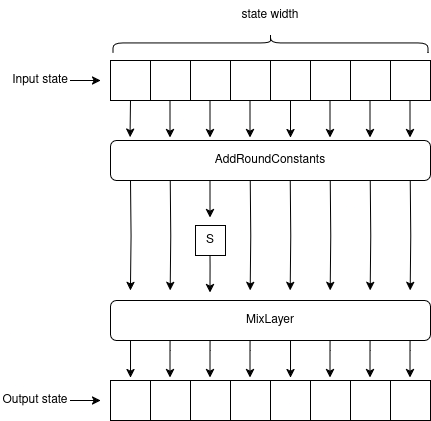
\includegraphics[width=\textwidth]{poseidon/partial.png}
      \captionsetup{margin={40pt,0pt}}
      \caption{\textsc{Hades} partial round.}\label{subfig:poseidonpartial}
    \end{subfigure}
    \hfill
    \begin{subfigure}{0.40\textwidth}
      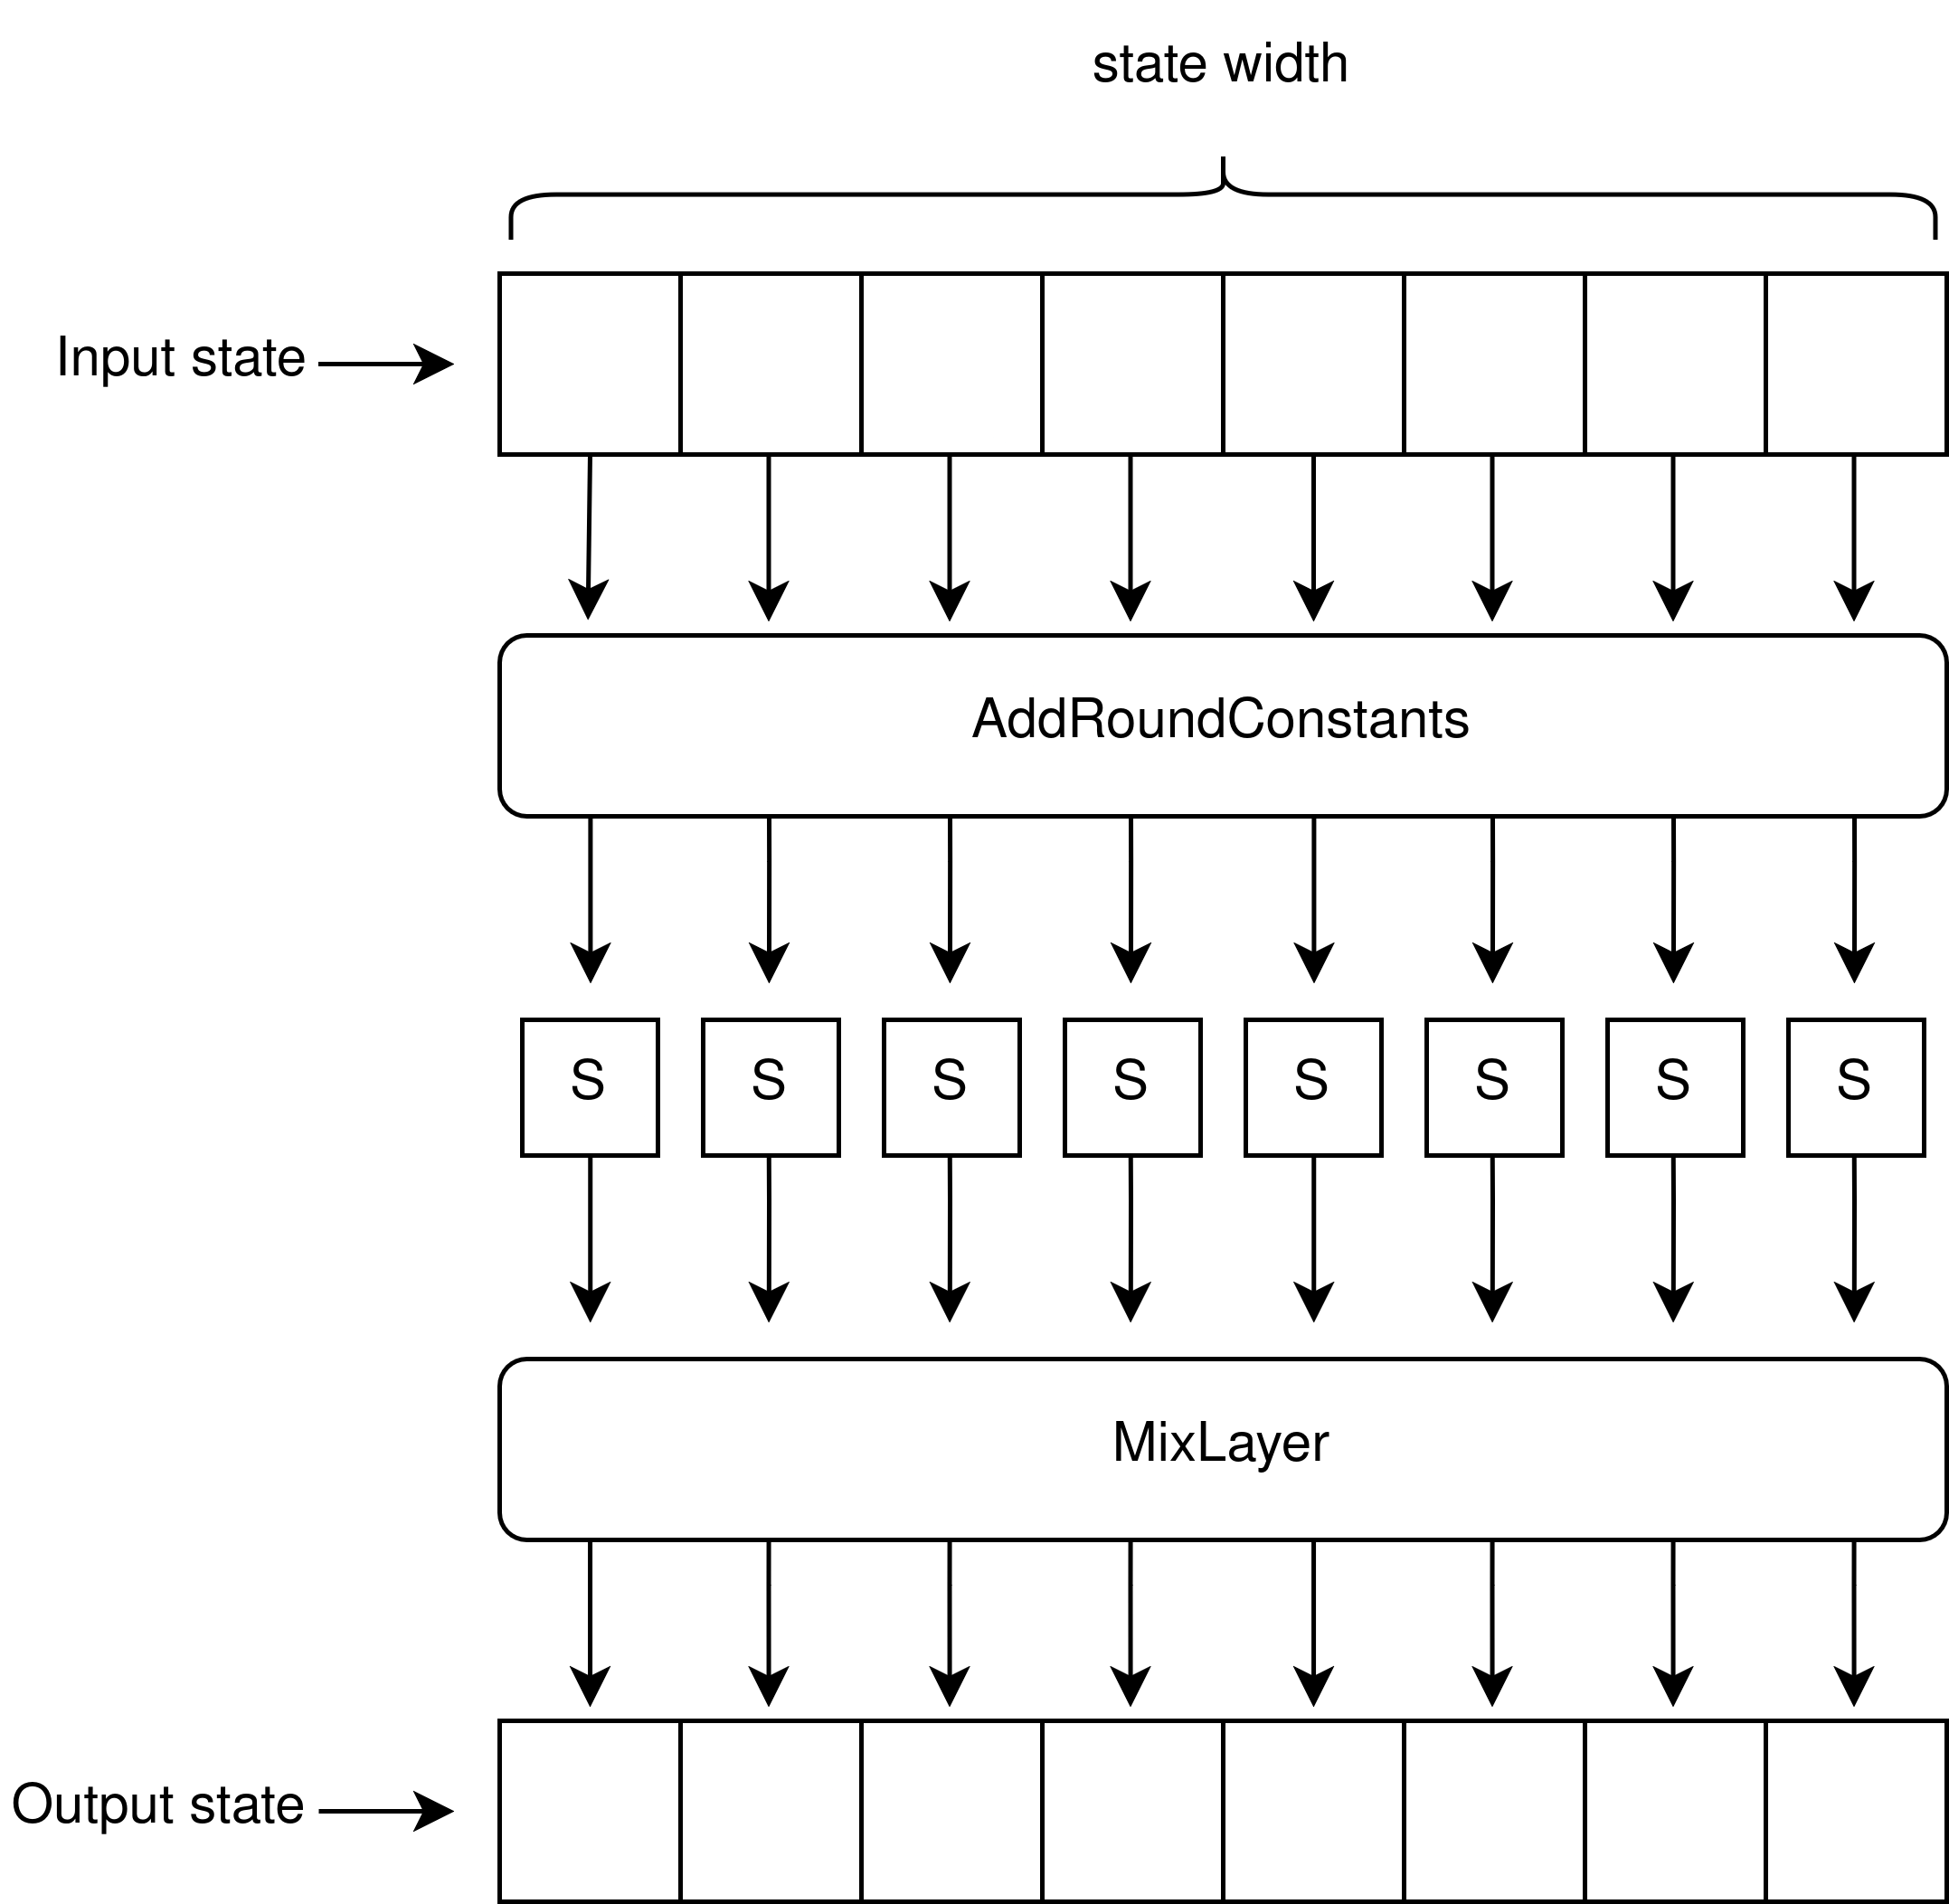
\includegraphics[width=\textwidth]{poseidon/full.png}
      \captionsetup{margin={40pt,0pt}}
      \caption{\textsc{Hades} full round.}\label{subfig:poseidonfull}
    \end{subfigure}
  \end{center}
\end{figure}
\renewcommand\thesubfigure{c}
\begin{figure}[H]
  \begin{center}
    \begin{subfigure}{0.40\textwidth}
      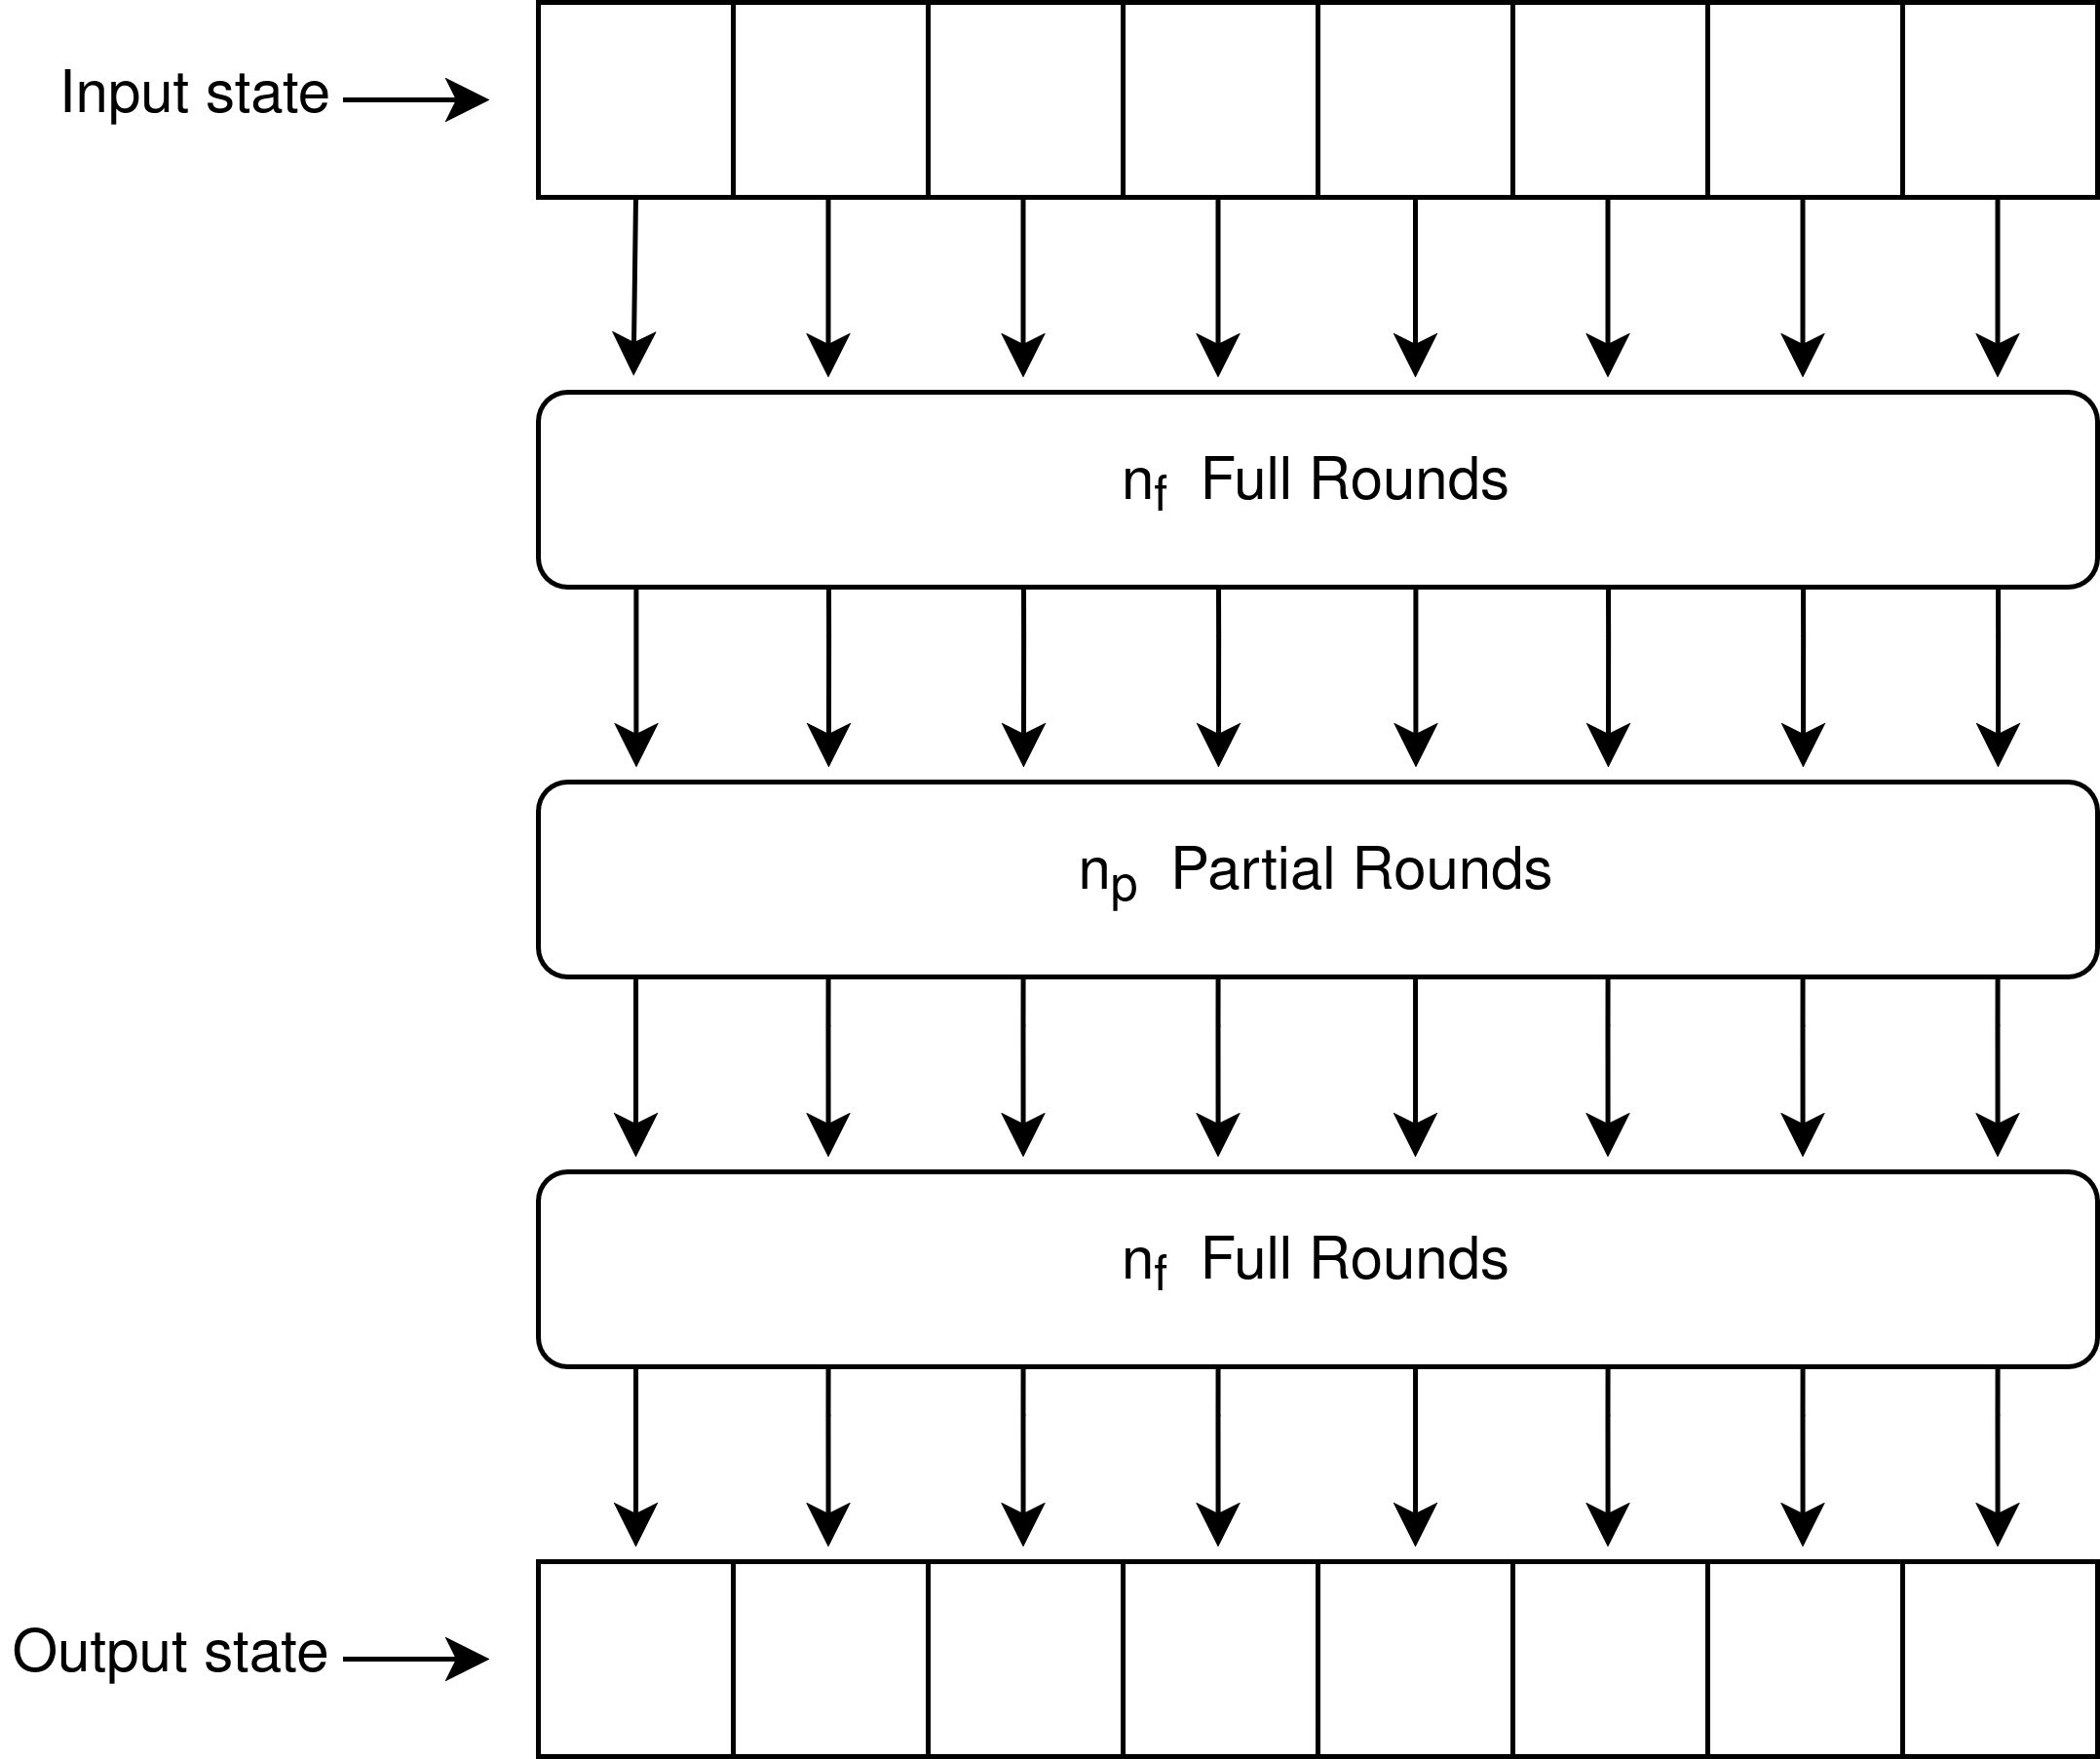
\includegraphics[width=\textwidth]{poseidon/structure.png}
      \captionsetup{margin={30pt,0pt}}
      \caption{Complete \textsc{Hades} function.}\label{subfig:poseidonstructure}
    \end{subfigure}
  \end{center}
  \caption{}\label{fig:poseidon}
\end{figure}

Some commonly used instantiations of \textsc{Poseidon} are shown here in Table~\ref{tab:poseidoninstances}:
\begin{table}[H]
  \begin{center}
    \begin{tabular}{|l|c|c|}
      \hline
      $t$ state width & 2/3 & 4/5/6/8 \\
      \hline
      $n_f$ full rounds & 8 & 8 \\
      \hline
      $n_p$ partial rounds & 57 & 60 \\
      \hline
    \end{tabular}
  \end{center}
  \caption{\textsc{Poseidon} instances.}\label{tab:poseidoninstances}
\end{table}

\subsection{\texttt{Rescue}}\label{subsec:rescue}

The \texttt{Rescue} primitive is a sponge function based on the \texttt{Marvellous} design strategy and the focus of the authors of this primitive was on the realization of a secure and robust function, rather than an efficient one, while keeping a simple structure.
For this reason is born the \texttt{Marvellous} strategy which is a SPN\footnote{Substitution-Permutation Network} round function, where each round is split into two phases and each phase is the composition of the different operations.

A single round is organized as follows:
\begin{itemize}
  \item \textbf{First phase}
  \begin{itemize}
    \item \textit{Inverse S-Box}: application of the inverse power map $x_i \rightarrow x_i^{-d}$ to each element of the state;
    \item \textit{MixLayer}: matrix-vector multiplication between an MDS matrix and the state;
    \item \textit{AddRoundConstant}: addition of a different constant to each element of the state, which also depends on the round and on the phase;
  \end{itemize}
  \item \textbf{Second phase}
  \begin{itemize}
    \item \textit{S-Box}: application of the power map $x_i \rightarrow x_i^d$ to each element of the state;
    \item \textit{MixLayer}: matrix-vector multiplication with the same MDS matrix of the first phase;
    \item \textit{AddRoundConstant}: addition of other different constants to the elements of the state.
  \end{itemize}
\end{itemize}

The round function is summarized in figure~\ref{fig:rescue}:
\begin{figure}[H]
  \begin{center}
    \includegraphics[width=0.40\textwidth]{rescue/round.png}
  \end{center}
  \caption{Single round of \texttt{Marvellous} permutation.}\label{fig:rescue}
\end{figure}

The most common instantiations of \texttt{Rescue} are shown in table~\ref{tab:rescueinstances}:
\begin{table}[H]
  \begin{center}
    \begin{tabular}{|l|c|c|c|c|}
      \hline
      $t$ state width & 3 & 4 & 5 & 6/8 \\
      \hline
      $n$ rounds & 14 & 11 & 9 & 8 \\
      \hline
    \end{tabular}
  \end{center}
  \caption{\texttt{Rescue} instances for $d = 5$.}\label{tab:rescueinstances}
\end{table}

\subsection{\texttt{Rescue-Prime}}\label{subsec:rescueprime}

The hash function \texttt{Rescue-Prime} has the same general underlying structure of \texttt{Rescue}~\ref{subsec:rescue}, but with minor adjustments to simplify the implementation, which are:
\begin{itemize}
  \item Simplification of the round constants' derivation function;
  \item Reduction of the security margin to its half (\textsl{i.e.} from $100\%$ to $50\%$);
  \item Flipping in the order of the S-Boxes.
\end{itemize}

The authors decided to not override the previous \texttt{Rescue} hash function, but to deploy these changes in a new version and to do so it has been decided to give it a new name to maintain a clear distinction between the two versions.
In fact, even the inner permutation function changed name to \texttt{Rescue-XLIX}\footnote{Rescue Forty-nine}.

The round function described for \texttt{Rescue} is still valid for \texttt{Rescue-Prime}, but with the changes mentioned above, \textsl{i.e.} inversion of the S-Boxes order.

Because the general structure is the same, also the number of rounds and state width are the same shown in table~\ref{tab:rescueinstances}.

\subsection{\textsc{Griffin}}\label{subsec:griffin}

This primitive, born from the results collected by the designs of \texttt{GMiMC} and \texttt{Rescue}, is the union of both SPN and Feistel networks schemes.
The structure on which \textsc{Griffin} has been built upon is called \textit{Horst} and is a revised version of Feistel networks, that grants a more robust defense against algebraic attacks \textsl{e.g.} Gr\"obner basis attacks.

The internal permutation function implemented for \textsc{Griffin} is called \textsc{Griffin-$\pi$} and has been designed to lower the minimum number of rounds while maintain a certain security level; this is achieved by the introduction of an exponentiation of very high degree on only one element of the state. This choice allows reducing the number of rounds without increasing too much the computational complexity and the number of constraints in the ZK proof.

A single round of the permutation function \textsc{Griffin-$\pi$} is organized as follows:
\begin{itemize}
  \item \textit{S-Box}: depending on the element's position, the transformation of the \textit{S-Box} is different and its formula is
  \begin{equation}
    y_i = \left\{
      \begin{array}{ll}
        x_0^{1/d} & \text{if } i = 0; \\
        x_1^{d} & \text{if } i = 1; \\
        x_i \cdot ((L_i^2 + \alpha_i \cdot L_i + \beta_i) & \text{otherwise}.
      \end{array}
    \right.
    \label{eq:griffinsbox}
  \end{equation}
  where
  \begin{equation}
    L_i = \left\{
      \begin{array}{ll}
        (i-1) \cdot y_0 + y_1 & \text{if } i = 2; \\
        (i-1) \cdot y_0 + y_1 + x_{i-1} & \text{otherwise}.
      \end{array}
    \right.
    \label{eq:griffinli}
  \end{equation}
  and $\alpha_i$,$\beta_i$ are constants generated \textsl{s.t.} $\alpha_i^2 - 4 \cdot \beta_i$ is a quadratic non-residue modulo $p$;
  \item \textit{MixLayer}: matrix-vector multiplication between an MDS fixed matrix and the state;
  \item \textit{AddRoundConstant}: a round constant that is equal for each element of the state, is added to the state.
\end{itemize}

The overall round function has been schematized in the following figure~\ref{fig:griffin}:
\begin{figure}[H]
  \begin{center}
    \includegraphics[width=0.25\textwidth]{griffin/round.png}
  \end{center}
  \caption{Single round of \textsc{Griffin-$\pi$} permutation.}\label{fig:griffin}
\end{figure}

Before computing the \textsc{Griffin-$\pi$} permutation function on the needed rounds, the state needs to be initialized with the application of the \textit{MixLayer} matrix-vector multiplication for an increased diffusion and better security.

Furthermore, the permutation \textsc{Griffin-$\pi$} can be used with \textsc{Griffin} in sponge as well as in a compression mode, interchangeably. 

In the table~\ref{tab:griffininstances} are provided the most common instantiations of \textsc{Griffin}:
\begin{table}[H]
  \begin{center}
    \begin{tabular}{|l|c|c|c|}
      \hline
      $t$ state width & 3 & 4 & 8 \\
      \hline
      $n$ rounds & 14 & 11 & 9 \\
      \hline
    \end{tabular}
  \end{center}
  \caption{\textsc{Griffin} instances for $d = 5$.}\label{tab:griffininstances}
\end{table}
where the minimum number of rounds $n$ is computed with the following formula:
\begin{equation}
  n \ge \left\lceil 1.2 \cdot \max \left\{6, \left\lceil \frac{2.5 \cdot \kappa}{\log_2(p) - \log_2(d-1)} \right\rceil, 1 + n_{GB} \right\} \right\rceil
  \label{eq:griffinrounds}
\end{equation}
with $\kappa$ the bits security level (in our case 128), $p$ the prime used for the curve, $d$ the exponent of the S-Box and $n_{GB}$ the number of rounds needed to defend against Gr\"obner basis attacks.

\subsection{\texttt{Anemoi}}\label{subsec:anemoi}

To improve the efficiency in terms of \textbf{evaluation} and \textbf{verification} of zero-knowledge proof's circuits, it has been proposed this new primitive based on \textbf{CCZ-equivalence} called \texttt{Anemoi}. It is a sponge function which inner permutation doesn't implement the usual S-Box structure, but instead a new design called \texttt{Flystel} which allows both a high degree evaluation and a low degree verification.
There are two types of \texttt{Flystel} gates, which are the open and the closed one and because are CCZ-equivalent, for this project it has been decided to implement only the open one with the documentation's proposed parameters to work in odd prime characteristic (figure~\ref{fig:flystel}), due to our prime $p$ choice.

\begin{figure}[H]
  \begin{center}
    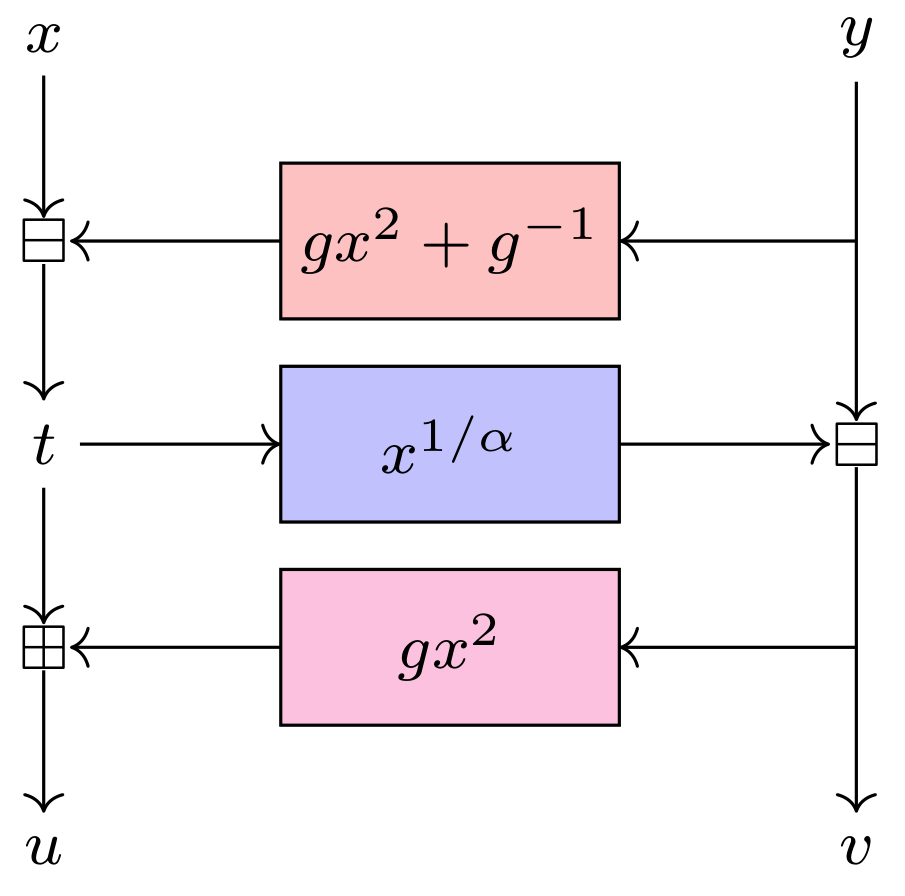
\includegraphics[width=0.25\textwidth]{anemoi/flystel.png}
  \end{center}
  \caption{$\texttt{Flystel}_p$ in odd prime characteristic.}\label{fig:flystel}
\end{figure}

The management of the state in the \texttt{Anemoi} round function is different from the previous primitives, because the state is divided into two halves, respectively called $x$ and $y$, for which the operations slightly differ.

The round is composed of the following steps:
\begin{itemize}
  \item \textit{AddRoundConstant}: addition of the round constants to both halves;
  \item \textit{MixLayer}: matrix-vector multiplication between a matrix $M_x$ and the $x$ half and also between matrix $M_y$ and the $y$ half, where $M_y$ is the row-permuted version of $M_x$;
  \item \textit{PHT~\footnote{Pseudo-Hadamard Transformation}}: application of the PHT to mix the two halves, which is defined as:
      \begin{gather}
        Y \leftarrow Y + X \\
        X \leftarrow X + Y
        \label{eq:pht}
      \end{gather}
  \item \textit{Flystel}: application of previously described open \texttt{Flystel} gate to the state.
\end{itemize}
and the visual representation is the following (figure~\ref{fig:anemoi}):
\begin{figure}[H]
  \begin{center}
    \includegraphics[width=0.40\textwidth]{anemoi/round.png}
  \end{center}
  \caption{Single round of the \texttt{Anemoi} permutation.}\label{fig:anemoi}
\end{figure}

The \texttt{Anemoi} permutation function works by iterating the round function for the needed number of rounds and finally compute an additional \textit{MixLayer} on the state.

The most common instantiations of this primitive are shown in the following table~\ref{tab:aneomiinstances}:

\begin{table}[H]
  \begin{center}
    \begin{tabular}{|l|c|c|c|}
      \hline
      $t$ state width & 2 & 4 & 6/8 \\
      \hline
      $n$ rounds & 21 & 14 & 12 \\
      \hline
    \end{tabular}
  \end{center}
  \caption{\texttt{Anemoi} instances for $d = 5$.}\label{tab:aneomiinstances}
\end{table}
and the number of rounds $n$ is computed with the following formula:
\begin{equation}
  n \ge \max \left\{ 8, \underbrace{\min \left\{ 5, l+1 \right\}}_{\text{security margin}} + \underbrace{\min \left\{ r \in \mathbb{N} | \mathcal{C}_{alg(r)} \ge 2 \right\} + 2}_{\text{security for algebraic attacks}} \right\}
  \label{eq:anemoirounds}
\end{equation}
where $l = \frac{t}{2}$ is the width of the halves and $t$ the total size of the state.

\subsection{\texttt{Arion}}\label{subsec:arion}

The last primitive implemented in this project is \texttt{Arion}, from which has been built the respective hash function named \texttt{ArionHash} and although it exists also an aggressive version, called \texttt{$\alpha$-Arion}, this has not been implemented in this project.
The permutation function inside \texttt{Arion} is different from the previous ones because is used the \textit{GTDS}\footnote{Generalized Triangular Dynamical System} structure, which is an alternative solution to the same approach used in the primitive \textsc{Griffin}, where the aim was to maintain a low multiplicative complexity and a low number of rounds, without affecting the security level.

A single round through \texttt{Arion} is computed with the following operations:
\begin{itemize}
  \item \textit{GTDS}: application of the GTDS structure to the state, which is defined as follows:
    \begin{equation}
      f_i(x_1, \ldots, x_t) = \left\{
          \begin{array}{ll}
            x_i^{d_1} \cdot g_i(\sigma_{i+1, n}) + h_i(\sigma_{i+1, n}) & \text{if } i < t; \\
            x_i^{e} & \text{if } i = t.
          \end{array}
        \right.
      \label{eq:gtds}
    \end{equation}
    where
    \begin{itemize}
      \item $t$ is the state width;
      \item $d_1$ the smallest positive integer co-prime with $p-1$;
      \item $e$ is the multiplicative inverse of $d_2$ modulo $p-1$, with $d_2$ coprime with $p-1$;
      \item the function $g_i(x)$ is:
        \begin{equation}
          g_i(x) = x^2 + \alpha_{i,1} \cdot x + \alpha_{i,2}
          \label{eq:g}
        \end{equation}
        with $\alpha_{i,1}$ and $\alpha_{i,2}$ constants that depend on the round;
      \item the function $h_i(x)$ is:
        \begin{equation}
          h_i(x) = x^2 + \beta_i \cdot x
          \label{eq:h}
        \end{equation}
        with $\beta_i$ a constant that depends on the round;
      \item and finally the parameter $\sigma_{i+1, n}$ is equal to:
        \begin{equation}
          \sigma_{i+1, n} = \sum_{j=i+1}^{t} x_j + f_j(x_1, \ldots, x_t)
          \label{eq:theta}
        \end{equation}
    \end{itemize}
  \item \textit{MixLayer}: matrix-vector multiplication between a fixed matrix and the state;
  \item \textit{AddRoundConstant}: addition of the round constant to each element of the state.
\end{itemize}
where, in the \texttt{Arion} documentation\cite{arion}, the last two operations are seen as a single layer called \textit{AffineLayer}.

The visual representation of a single round is shown below (figure~\ref{fig:arion}):

\begin{figure}[H]
  \begin{center}
    \includegraphics[width=0.25\textwidth]{arion/round.png}
  \end{center}
  \caption{Single round of the \texttt{Arion} permutation.}\label{fig:arion}
\end{figure}

Furthermore, a complete permutation in \texttt{Arion} is done with an initial application of the \textit{MixLayer} to the state and then the iteration of the round function for the number of rounds needed.
The most common instantiations of \texttt{Arion} are shown in table~\ref{tab:aneomiinstances}:
\begin{table}[H]
  \begin{center}
    \begin{tabular}{|l|c|c|c|}
      \hline
      $t$ state width & 3 & 4/5/6 & 8 \\
      \hline
      $n$ rounds & 6 & 5 & 4 \\
      \hline
    \end{tabular}
  \end{center}
  \caption{\texttt{Arion} instances for $d_1 = 5$.}\label{tab:aneomiinstances}
\end{table}

\section{Implementation}\label{sec:implementation}

All the code that has been used to perform the tests over the implemented primitives is hosted the following GitHub repository \url{https://github.com/Crisis82/AOHashes}.

The structure of the repository follows the standard hierarchy structure of a Rust project managed with \textbf{Cargo}, thus the folders are organized as follows:
\begin{itemize}
  \item \textit{benches}: it contains the tests used to measure the performances of the primitives, whose results are collected in this paper (see chapter~\ref{chap:tests});
  \item \textit{docs}: it contains the official documentation used to implement the primitives and this paper;
  \item \textit{examples}: it contains a simple usage example to deploy the primitives;
  \item \textit{src}: it contains almost all the code of the project, especially the implementation of the primitives which are contained under the \textit{permutation} subdirectory;
  \item \textit{tests}: it contains the code used to perform the tests for the verification of the correctness of the primitives.
\end{itemize}

For each primitive it has been decided to create two separate modes:
\begin{enumerate}
  \item plain hash function: this has been implemented in the files called \texttt{scalar.rs} and works with values in the BLS12-381 curve;
  \item zero-knowledge proof generation and verification: inside the \texttt{gadget.rs} files have been implemented the operations of the permutation's functions that work with the \textsf{Plonk} constraint system.
\end{enumerate}
plus for each function there is a file \texttt{hash\_name.rs} (\textsl{e.g.} \texttt{gmimc.rs}) that defines the permutation and a \texttt{params.rs} which dynamically generates the parameters needed, like exponents, constants or matrices, by the permutation function.

It has been decided for a dynamical approach for the parameters' generation for two reasons:
\begin{enumerate}
  \item follows the elastic nature of AO primitives;
  \item better reliability in the parameters generated values, removing the constant worry of having not updated the parameters for the given instances.
\end{enumerate}

\begin{note}
  During the parameters' implementation process, it has been found out that the method provided and suggested by the Dusk Network team for passing the constants and the MDS matrix was faulty, because the generated values were not the same of the ones written on the file.
\end{note}

\subsection{Execution}\label{subsec:execution}

Thanks to Cargo, the execution of tests or benchmarks is straightforward, via these commands:
\begin{lstlisting}[language=bash]
  # for executing tests
  cargo test --features={hash_name},zk,encryption

  # for executing benchmarks
  cargo bench --features={hash_name},zk,encryption
\end{lstlisting}
The above shell commands execute respectively a test or a benchmark on the \textit{hash\_name} primitive provided on all possible evaluations: plain computation, encryption/decryption and zero-knowledge proof.
However, is possible to change the evaluation types just by passing as feature only \texttt{zk} or \texttt{encryption} along with the hash function name.
Additionally, for the benchmarks is even possible to evaluate just 1 of the 3 benchmarks available (\textit{encrypt}, \textit{decrypt} or \textit{hash}), for example
\begin{lstlisting}[language=bash]
  cargo bench hash --features=gmimc,zk
\end{lstlisting}
runs the test on the \texttt{GMiMC} hash function over \textit{plain} and \textit{zero-knowledge} evaluations, but it does not test the encryption or decryption functions.

\chapter{Tests}\label{chap:tests}

The tests that will be presented in this chapter are divided into four categories, in order to have a complete comparison between the primitives and highlight the point of strength and weakness of each one:
\begin{enumerate}
  \item \textit{Plain performance}: the time of computation of the final digest working with scalar values in the BLS12-381 curve, measured in $\mu s$;
  \item Number of \textit{constraints}: the number of constraints needed by the primitive to generate a complete \textsf{Plonk} proof, which gives an idea of the computational cost of the proof;
  \item Zero-Knowledge \textit{proof generation}: the time needed to generate a proof measured in $ms$;
  \item Zero-Knowledge \textit{proof verification}: the time needed to verify the generated proof measured in $ms$;
\end{enumerate}

All the tests have been performed on the same machine, with the following specifications:
\begin{table}[H]
    \centering
    \begin{tabular}{|c||c|}
      \hline
        CPU & AMD Ryzen 5 3600 \\
        GPU & NVIDIA GeForce RTX 2060 \\
        RAM & 16GB \\
        OS & Void Linux x86\_64 \\
        \hline
        Rustup & 1.27.1 \\
        Rustc & 1.85.0-nightly \\
        Cargo & 1.85.0-nightly \\
      \hline
    \end{tabular}
    \label{tab:machinespecs}
\end{table}
All the other cargo dependencies used with their versions are listed in the \texttt{Cargo.toml} file inside the project.

Furthermore, to have a fair comparison, any possible optimization proposed by the authors of the primitives has \textbf{not} been implemented and for this reason has been removed also the one implemented in the \textsc{Poseidon} primitive for state width $t = 5$.
In this way, equal operations have the same computational complexity and an equal number of constraints, allowing a reliable comparison in the tests results.

The exponent used in the power map by the S-Box for all primitives is $d = 5$, which is the smallest integer co-prime with $p-1$ for our choice of $p$ (see chapter~\ref{chap:overview}).
Additionally, each test has been performed for only one primitive at a time without having other programs running in the machine to avoid any possible interference.

Finally, to achieve a certain precision in the results, for each input sample and choice of parameters for the primitive, have been performed 1000 tests.
This process has been automated with the adoption of the crate (cargo library) \texttt{criterion} and the shell command used to execute each test is:
\begin{lstlisting}[language=bash]
  cargo bench hash --features={hash_name},zk
\end{lstlisting}
It is important to notice that if the reader wants to reproduce the tests, this command alone isn't enough because it has to pay attention to the choice of the maximum evaluation time for \texttt{criterion}, otherwise if a primitive is much slower that the others, the tests will be cut off before iterating all the 1000 tests, possibly leading to wrong results.

\begin{note}
  This note is here to remind the reader that not all primitives are built to work on all the tested state widths, that's why there will be some empty cells in the following presented tables.
\end{note}

\section{Plain performance}\label{sec:plain}

The first test that we wanted to analyze was the raw performance of the primitives to compute a hash digest, thus working with values in our chosen curve, rather than polynomial constraints.

In the following table~(\ref{tab:plain}) have been collected the average times of the results for this testing category, expressed in $\mu s$:

\begin{table}[H]
  \begin{center}
    \begin{tabular}{|l|c|c|c|c|c|}
      \hline
        state width & 3 & 4 & 5 & 6 & 8 \\
      \hline
        \texttt{Anemoi} & & 663 &  & 428 & 573 \\
        \texttt{Arion} & 530 & 606 & 385 & 467 & 508 \\
        \texttt{GMiMC} & 43 & 45 & \cellcolor{green!35} 24 & 26 & 30 \\
        \textsc{Griffin} & 549 & 440 & & & 198 \\
        \textsc{Poseidon} & 46 & 77 & 56 & 78 & 133 \\
        \texttt{Rescue} & \cellcolor{orange!35} 1641 & \cellcolor{orange!35} 1715 & 879 & 943 & \cellcolor{orange!35} 1264 \\
        \texttt{Rescue-Prime} & \cellcolor{orange!35} 1631 & \cellcolor{red!35} 1719 & 878 & 940 &  \cellcolor{orange!35} 1261 \\
      \hline
    \end{tabular}
  \end{center}
  \caption{Plain timing performance in $\mu s$ with $d = 5$.}\label{tab:plain}
\end{table}

And all the above results have been plotted in the following figure~\ref{plot:plain}, to have also a visual comparison between the timings.

Note that for the sake of clarity of the plot, the color of \texttt{Rescue} and \texttt{Rescue-Prime} is the same, due to the fact that their timings are very close.

\begin{figure}[H]
  \hspace{60pt}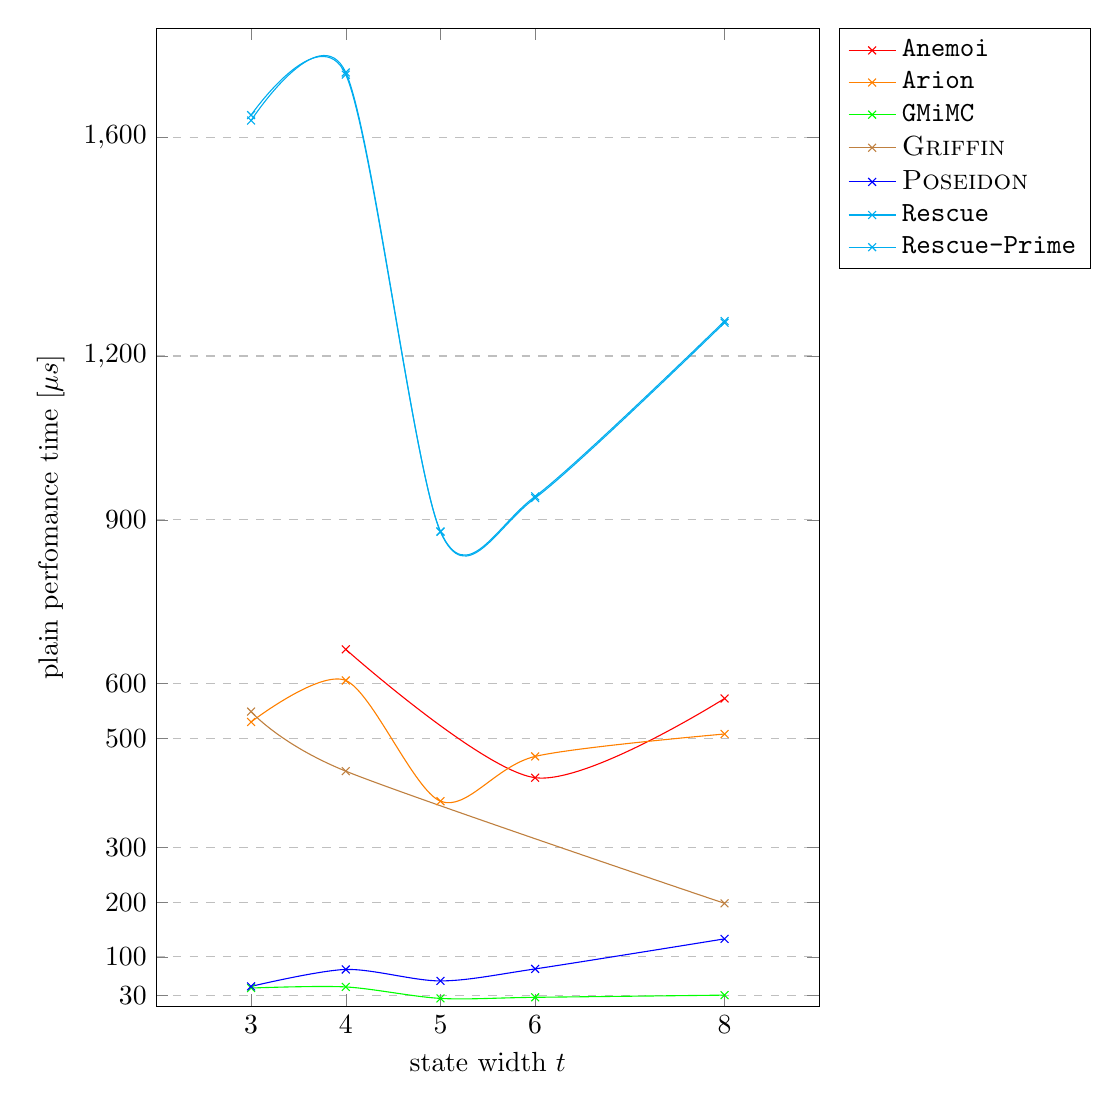
\begin{tikzpicture}
  \begin{axis}[
      xlabel={state width $t$},
      ylabel={plain perfomance time [$\mu s$]},
      ymajorgrids=true,
      grid style=dashed,
      width=10cm, height=14cm,
      xmin=2, xmax=9,
      ymin=10, ymax=1800,
      xtick={3,4,5,6,8}, ytick={30,100,200, 300, 500, 600, 900, 1200, 1600},
      legend pos=outer north east, legend cell align=left,
      smooth,
    ]

    % Anemoi
    \addplot[mark=x, color=red] plot coordinates {
        (4,663)
        (6,428)
        (8,573)
    };
    \addlegendentry{\texttt{Anemoi}}
    
    % Arion
    \addplot[mark=x, color=orange] plot coordinates {
        (3,530)
        (4,606)
        (5,385)
        (6,467)
        (8,508)
    };
    \addlegendentry{\texttt{Arion}}
    
    % GMiMC
    \addplot[mark=x, color=green] plot coordinates {
        (3,43)
        (4,45)
        (5,24)
        (6,26)
        (8,30)
    };
    \addlegendentry{\texttt{GMiMC}}
    
    \addplot[mark=x, color=brown] plot coordinates {
        (3,549)
        (4,440)
        (8,198)
    };
    \addlegendentry{\textsc{Griffin}}
    
    \addplot[mark=x, color=blue] plot coordinates {
        (3,46)
        (4,77)
        (5,56)
        (6,78)
        (8,133)
    };
    \addlegendentry{\textsc{Poseidon}}
    
    \addplot[mark=x, color=cyan] plot coordinates {
        (3,1641)
        (4,1715)
        (5,879)
        (6,943)
        (8,1264)
    };
    \addlegendentry{\texttt{Rescue}}
    
    \addplot[mark=x, color=cyan] plot coordinates {
        (3,1631)
        (4,1719)
        (5,878)
        (6,940)
        (8,1261)
    };
    \addlegendentry{\texttt{Rescue-Prime}}

  \end{axis}
\end{tikzpicture}

  \caption{Plain timing performance in $\mu s$ with $d = 5$.}\label{plot:plain}
\end{figure}

As it is possible to notice by the result's table, but even more in the plot, the fastest primitive is \texttt{GMiMC}, immediately followed by \textsc{Poseidon} and this is due to the fact that the design of these two primitives is based on keeping the computational cost of each round very low, using only low degree exponentiation in the S-Box, while having a high number of rounds.
However, the high number of rounds doesn't affect that much the performance, especially in the case of \texttt{GMiMC}, where the timings are pretty much the same for each state width.

It is also interesting the behavior of \textsc{Griffin}, in which the bigger is the state the faster is the computation and the reason behind this is that it's only done one high degree permutation per round, thus having a bigger state doesn't really affect the management of the state, while on the other hand the number of rounds is slightly lower, reducing the overall computational cost.

The remaining primitives (\texttt{Anemoi}, \texttt{Arion}, \texttt{Rescue} and \texttt{Rescue-Prime}) have an inconsistent and swinging behavior, especially \texttt{Rescue} and \texttt{Rescue-Prime}.

\section{Constraints}\label{sec:constraints}

For the second testing phase it has been analyzed the number of constraints needed both for a single round and for an entire permutation.
We analyzed also this aspect for the zero-knowledge evaluation, in order to have another point of view on the performance of the primitive other than the timings, that are exposed in the following tests sections (\ref{sec:proofgen}) (\ref{sec:proofver}).

The general formulas to calculate the number of constraints for a single round of each primitive are the following:

\begin{align*}
  \texttt{Anemoi}_{c_r} & = c_{\text{AddRoundConstant}} + c_{\text{MixLayer}} + c_{\text{PHT}} + c_{\text{S-Box}} =\\
    &= 2l + 2l^2 + 2l + 6l = 2l^2 + 10l =\\
    &= \frac{t^2}{2} + 5t\\[20pt]
  \texttt{Arion}_{c_r} &= c_{\text{GTDS}} + c_{\text{MixLayer}} + c_{\text{AddRoundConstant}} =\\
    &= (t-1) \cdot 7 + 16 + t + t^2 =\\
    &= t^2 + 8t + 9\\[20pt]
  \texttt{GMiMC}_{c_r} &= c_{\text{ERF}} = t+2\\[20pt]
  \textsc{Griffin}_{c_r} &= c_{\text{S-Box}} + c_{\text{MixLayer}} + c_{\text{AddRoundConstant}} =\\
    & = 6 + (t-2)*3 + t^2 + t =\\
    & = t^2 + 4t\\[20pt]
  \textsc{Poseidon}_{c_{partial}} &= c_{\text{AddRoundConstant}} + c_{\text{S-Box}} + c_{\text{MixLayer}} =\\
    &= t + 3 + t^2\\[20pt]
  \textsc{Poseidon}_{c_{full}} &= c_{\text{AddRoundConstant}} + c_{\text{S-Box}} + c_{\text{MixLayer}} =\\ 
    &= t + 3t + t^2 =\\
    &= t^2 + 4t\\[20pt]
  \texttt{Rescue}_{c_r} &= 2 \cdot (c_{\text{S-Box}} + c_{\text{MixLayer}} + c_{\text{AddRoundConstant}}) =\\
    &= 2 \cdot (3t + t^2 + t) =\\
    &= 2t^2 + 8t\\[20pt]
  \texttt{Rescue-Prime}_{c_r} &= 2 \cdot (c_{\text{S-Box}} + c_{\text{MixLayer}} + c_{\text{AddRoundConstant}}) =\\
    &= 2 \cdot (3t + t^2 + t) =\\
    &= 2t^2 + 8t
\end{align*}

We used the variable $c_r$ to denote the constraints per round.

Additionally, because of \textsc{Poseidon}'s design, where a round can be full or partial, we decided to show the number of constraints for both, round types and that's why for each cell there are two values, presented with the following notation \{partial\}/\{full\}.

\begin{table}[H]
  \begin{center}
    \begin{tabular}{|l|c|c|c|c|c|}
      \hline
        state width & 3 & 4 & 5 & 6 & 8 \\
      \hline
        \texttt{Anemoi} & & 28 &  & 48 & 72 \\
        \texttt{Arion} & 42 & 57 & 74 & 93 & \cellcolor{orange!35} 137 \\
        \texttt{GMiMC} & \cellcolor{green!35} 5 & 6 & 7 & 8 & 10 \\
        \textsc{Griffin} & 21 & 32 & & & 96 \\
        \textsc{Poseidon} & 15/21 & 23/32 & 33/45 & 45/60 & 75/96 \\
        \texttt{Rescue} & 42 & 64 & 90 & \cellcolor{orange!35} 120 & \cellcolor{red!35} 192 \\
        \texttt{Rescue-Prime} & 42 & 64 & 90 & \cellcolor{orange!35} 120 & \cellcolor{red!35} 192 \\
      \hline
    \end{tabular}
  \end{center}
  \caption{Number of constraints needed for a single round of the permutation with $d = 5$.}\label{tab:constraintsround}
\end{table}

Now we extend the above results to an entire permutation, thus we define $c_p$ as constraints per permutation and define the general formulas:
\begin{align*}
  \texttt{Anemoi}_{c_p} &= \texttt{Anemoi}_{c_r} * n + c_{\text{MixLayer}} = \texttt{Anemoi}_{c_r} * n + 2l^2 \\[20pt]
  \texttt{Arion}_{c_p} &= \texttt{Arion}_{c_r} * n + c_{\text{MixLayer}} = \texttt{Arion}_{c_r} * n + t^2 \\[20pt]
  \texttt{GMiMC}_{c_p} &= \texttt{GMiMC}_{c_r} * n \\[20pt]
  \textsc{Griffin}_{c_p} &= \textsc{Griffin}_{c_r} * n + c_{\text{MixLayer}} = \textsc{Griffin}_{c_r} * n + t^2 \\[20pt]
  \textsc{Poseidon}_{c_p} &= \textsc{Poseidon}_{c_{partial}} * n_p + \textsc{Poseidon}_{c_{full}} * n_f \\[20pt]
  \texttt{Rescue}_{c_p} &= \texttt{Rescue}_{c_r} * n \\[20pt]
  \texttt{Rescue-Prime}_{c_p} &= \texttt{Rescue-Prime}_{c_r} * n
\end{align*}

\begin{table}[H]
  \begin{center}
    \begin{tabular}{|l|c|c|c|c|c|}
      \hline
        state width & 3 & 4 & 5 & 6 & 8 \\
      \hline
        \texttt{Anemoi} & & 400 & & 594 & 896 \\
        \texttt{Arion} & \cellcolor{green!35} 261 & 301 & 395 & 501 & 612 \\
        \texttt{GMiMC} & \cellcolor{orange!35} 1640 & \cellcolor{orange!35} 1980 & \cellcolor{orange!35} 2324 & \cellcolor{orange!35} 2672 & \cellcolor{orange!35} 3380 \\
        \textsc{Griffin} & 303 & 368 & & & 928 \\
        \textsc{Poseidon} & \cellcolor{orange!35} 1317 & \cellcolor{orange!35} 2104 & \cellcolor{orange!35} 2964 & \cellcolor{orange!35} 3960 & \cellcolor{red!35} 6360 \\
        \texttt{Rescue} & 588 & 704 & 810 & 960 & \cellcolor{orange!35} 1536 \\
        \texttt{Rescue-Prime} & 588 & 704 & 810 & 960 & \cellcolor{orange!35} 1536 \\
      \hline
    \end{tabular}
  \end{center}
  \caption{Number of constraints needed for a complete permutation with $d = 5$.}\label{tab:constraintsperm}
\end{table}

Even though \texttt{Rescue} and \texttt{Rescue-Prime} were the two primitives with the highest number of constraints per round, if we consider the entire permutation, which is the most important aspect, these two are still in the top 3 for the highest number of constraints, but not as much as \texttt{GMiMC} and \textsc{Poseidon}.
Is immediately clear that \textsc{Poseidon} is worst in terms of number of constraints per permutation because it was already among the worst primitives considering only a round, but if we take into account its design strategy, it's obvious that the number of constraints per permutations increase exponentially due to its high number of rounds.

Furthermore, even though \texttt{GMiMC} is the second worst's primitive, it's not a bad result considering that the number of rounds needed by \texttt{GMiMC} is almost double of those needed by \textsc{Poseidon}.

On the other hand, thanks to its design that allow to keep the number of rounds very low, \texttt{Arion} is the best primitive in terms of constraints per permutation, even though it wasn't the best in terms of constraints per round.

\section{Proof generation}\label{sec:proofgen}

In the third tests type, we focused on the time needed to generate a zero-knowledge proof with the Plonk constraint system, which we have collected in the following table~(\ref{tab:proofgen}):

\begin{table}[H]
  \begin{center}
    \begin{tabular}{|l|c|c|c|c|c|}
      \hline
        state width & 3 & 4 & 5 & 6 & 8 \\
      \hline
        \texttt{Anemoi} & & 657 &  & 656 & 658 \\
        \texttt{Arion} & 358 & 660 & 356 & \cellcolor{green!35} 355 & 657 \\
        \texttt{GMiMC} & \cellcolor{orange!35} 1959 & \cellcolor{orange!35} 1956 & \cellcolor{orange!35} 1955 & \cellcolor{orange!35} 1966 & \cellcolor{orange!35} 1966 \\
        \textsc{Griffin} & 655 & 657 & & & 660 \\
        \textsc{Poseidon} & \cellcolor{orange!35} 1958 & \cellcolor{orange!35} 1961 & \cellcolor{orange!35} 1973 & \cellcolor{orange!35} 1959 & \cellcolor{red!35} 3719 \\
        \texttt{Rescue} & \cellcolor{orange!35} 1221 & \cellcolor{orange!35} 1212 & 659 & 664 & \cellcolor{orange!35} 1219 \\
        \texttt{Rescue-Prime} & \cellcolor{orange!35} 1212 & \cellcolor{orange!35} 1219 & 659 & 659 & \cellcolor{orange!35} 1213 \\
      \hline
    \end{tabular}
  \end{center}
  \caption{Proof generation performance's time in $ms$ with $d = 5$.}\label{tab:proofgen}
\end{table}

And the following figure~(\ref{plot:proofgen}) corresponds to the above data that have been plotted, to have also a visual comparison between the different primitives:

\begin{figure}[H]
  \hspace{60pt}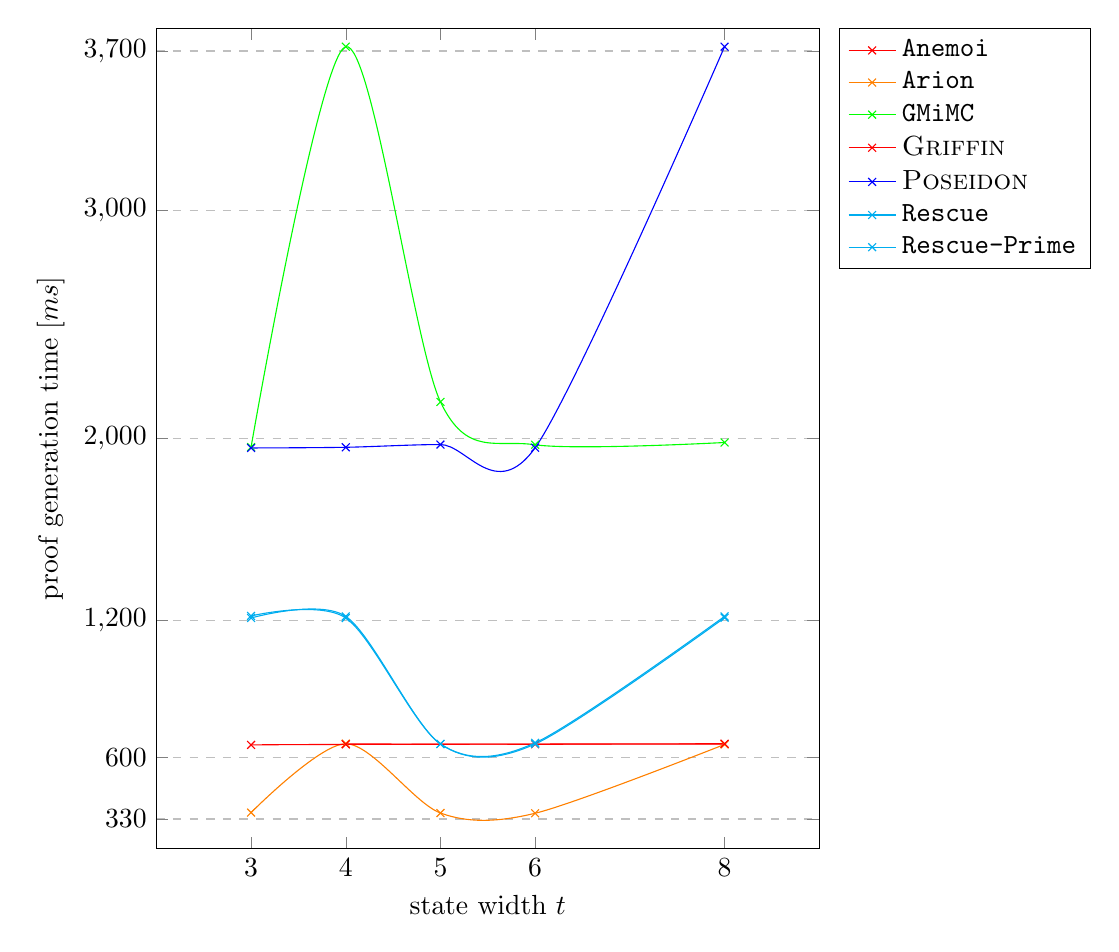
\begin{tikzpicture}
  \begin{axis}[
      xlabel={state width $t$},
      ylabel={proof generation time [$ms$]},
      ymajorgrids=true,
      grid style=dashed,
      width=10cm, height=12cm,
      xmin=2, xmax=9,
      ymin=200, ymax=3800,
      xtick={3,4,5,6,8}, ytick={330,600,1200,2000,3000, 3700},
      legend pos=outer north east, legend cell align=left,
      smooth,
    ]
      
    % Anemoi
    \addplot[mark=x, color=red] plot coordinates {
        (4,659)
        (6,658)
        (8,659)
    };
    \addlegendentry{\texttt{Anemoi}}
    
    % Arion
    \addplot[mark=x, color=orange] plot coordinates {
        (3,358)
        (4,660)
        (5,356)
        (6,355)
        (8,657)
    };
    \addlegendentry{\texttt{Arion}}
    
    % GMiMC
    \addplot[mark=x, color=green] plot coordinates {
        (3,1962)
        (4,3719)
        (5,2160)
        (6,1972)
        (8,1982)
    };
    \addlegendentry{\texttt{GMiMC}}
    
    \addplot[mark=x, color=red] plot coordinates {
        (3,655)
        (4,657)
        (8,660)
    };
    \addlegendentry{\textsc{Griffin}}
    
    \addplot[mark=x, color=blue] plot coordinates {
        (3,1958)
        (4,1961)
        (5,1973)
        (6,1959)
        (8,3719)
    };
    \addlegendentry{\textsc{Poseidon}}
    
    \addplot[mark=x, color=cyan] plot coordinates {
        (3,1221)
        (4,1212)
        (5,659)
        (6,664)
        (8,1219)
    };
    \addlegendentry{\texttt{Rescue}}
    
    \addplot[mark=x, color=cyan] plot coordinates {
        (3,1212)
        (4,1219)
        (5,659)
        (6,659)
        (8,1213)
    };
    \addlegendentry{\texttt{Rescue-Prime}}

  \end{axis}
\end{tikzpicture}

  \caption{Proof generation performance's time in $ms$ with $d = 5$.}\label{plot:proofgen}
\end{figure}

For a better understanding of the results, we decided to assign the same color to \texttt{Anemoi} and \textsc{Griffin} and also to \texttt{Rescue} and \texttt{Rescue-Prime}, because their timings are so close that their curves are overlapping.

As it is possible to evince from these results, the fastest primitive for this category of tests is \texttt{Arion}, immediately followed by \texttt{Anemoi} and \textsc{Griffin}.
Nonetheless, considering that the latest two primitives works only with 3 out 5 possible state widths, their results is almost as good as \texttt{Arion}.
If we have to take also in consideration the stability of the results, \texttt{Arion} is a little unstable and whose behavior is closely related to the one of the plain performance test.

On the other spectrum of the tests' results, \textsc{Poseidon} is the worst primitive in terms of proof generation as expected by the high number of constraints per permutation highlighted in the previous section (\ref{sec:constraints}), almost doubling the time in the case of state width $t = 8$ respectively to average time of the other state widths' values.

\section{Proof verification}\label{sec:proofver}

In the last category of tests, we focused on the verification process of the constraint generated in the Plonk system, and the results have been pretty much the same, around $7.26\pm0.03\ [ms]$ independently of the state width, for all the primitives.
Due to these results, it has been decided to not show any table or plot like in the previous sections.

\chapter{Conclusion}\label{chap:conclusion}

In conclusion, as it was possible to deduct from the tests, the design strategy for primitives plays a key role in how the function behaves with different parameters, highlighting the strengths and weaknesses of each one.
This is a crucial step before proceeding with the optimization of these permutation functions, because it's beneficial to decide which applications can fit better the behavior of the primitive, not only from a performance standpoint, but even more from a security one.
For example, even though \texttt{Arion} is the fastest for a certain choice of parameters, it leads to the same results of \texttt{Anemoi} and \textsc{Griffin} for others, thus if an application needs among the requirements also a certain level of stability in the performances while providing a broader choice of parameters, going with \texttt{Arion} would not be the best choice.
On the other hand, while \texttt{GMiMC} has been one of the first primitives that animated some interest in AO cryptography, thus one may think that its performance will not be as good as the newly proposed primitives, if the area of application needs a higher number of hashes computations without the constant need of zero-knowledge proofs, \texttt{GMiMC} would be the best choice.

We hope that with this paper we have provided a good overview of the current state of the AO primitives and that with these results new optimizations may come out, or even better that this will spark new ideas for innovative design strategies that will enrich the cryptographic community.

\nocite{*}
\printbibliography[heading=bibnumbered,title={References}]

\end{document}
